% Created by tikzDevice version 0.7.0 on 2014-07-31 11:04:53
% !TEX encoding = UTF-8 Unicode
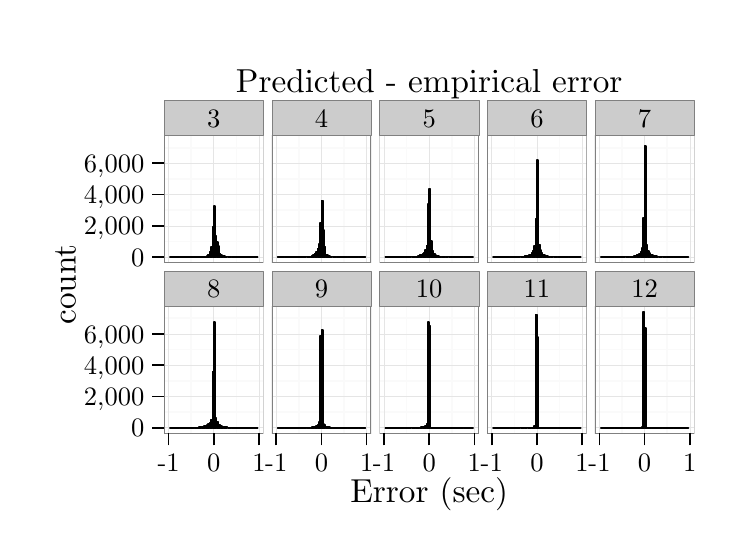
\begin{tikzpicture}[x=1pt,y=1pt]
\definecolor[named]{fillColor}{rgb}{1.00,1.00,1.00}
\path[use as bounding box,fill=fillColor,fill opacity=0.00] (0,0) rectangle (252.94,180.67);
\begin{scope}
\path[clip] (  0.00,  0.00) rectangle (252.94,180.67);
\definecolor[named]{drawColor}{rgb}{1.00,1.00,1.00}
\definecolor[named]{fillColor}{rgb}{1.00,1.00,1.00}

\path[draw=drawColor,line width= 0.6pt,line join=round,line cap=round,fill=fillColor] ( -0.00,  0.00) rectangle (252.95,180.67);
\end{scope}
\begin{scope}
\path[clip] ( 49.28, 95.69) rectangle ( 85.20,141.71);
\definecolor[named]{fillColor}{rgb}{1.00,1.00,1.00}

\path[fill=fillColor] ( 49.28, 95.69) rectangle ( 85.20,141.71);
\definecolor[named]{drawColor}{rgb}{0.98,0.98,0.98}

\path[draw=drawColor,line width= 0.6pt,line join=round] ( 49.28,103.43) --
	( 85.20,103.43);

\path[draw=drawColor,line width= 0.6pt,line join=round] ( 49.28,114.72) --
	( 85.20,114.72);

\path[draw=drawColor,line width= 0.6pt,line join=round] ( 49.28,126.01) --
	( 85.20,126.01);

\path[draw=drawColor,line width= 0.6pt,line join=round] ( 49.28,137.30) --
	( 85.20,137.30);

\path[draw=drawColor,line width= 0.6pt,line join=round] ( 59.08, 95.69) --
	( 59.08,141.71);

\path[draw=drawColor,line width= 0.6pt,line join=round] ( 75.40, 95.69) --
	( 75.40,141.71);
\definecolor[named]{drawColor}{rgb}{0.90,0.90,0.90}

\path[draw=drawColor,line width= 0.2pt,line join=round] ( 49.28, 97.79) --
	( 85.20, 97.79);

\path[draw=drawColor,line width= 0.2pt,line join=round] ( 49.28,109.07) --
	( 85.20,109.07);

\path[draw=drawColor,line width= 0.2pt,line join=round] ( 49.28,120.36) --
	( 85.20,120.36);

\path[draw=drawColor,line width= 0.2pt,line join=round] ( 49.28,131.65) --
	( 85.20,131.65);

\path[draw=drawColor,line width= 0.2pt,line join=round] ( 50.92, 95.69) --
	( 50.92,141.71);

\path[draw=drawColor,line width= 0.2pt,line join=round] ( 67.24, 95.69) --
	( 67.24,141.71);

\path[draw=drawColor,line width= 0.2pt,line join=round] ( 83.57, 95.69) --
	( 83.57,141.71);
\definecolor[named]{drawColor}{rgb}{0.00,0.00,0.00}
\definecolor[named]{fillColor}{rgb}{0.75,0.75,0.75}

\path[draw=drawColor,line width= 0.6pt,line join=round,fill=fillColor] ( 51.39, 97.79) rectangle ( 51.88, 97.79);

\path[draw=drawColor,line width= 0.6pt,line join=round,fill=fillColor] ( 51.88, 97.79) rectangle ( 52.38, 97.79);

\path[draw=drawColor,line width= 0.6pt,line join=round,fill=fillColor] ( 52.38, 97.79) rectangle ( 52.87, 97.79);

\path[draw=drawColor,line width= 0.6pt,line join=round,fill=fillColor] ( 52.87, 97.79) rectangle ( 53.37, 97.79);

\path[draw=drawColor,line width= 0.6pt,line join=round,fill=fillColor] ( 53.37, 97.79) rectangle ( 53.86, 97.79);

\path[draw=drawColor,line width= 0.6pt,line join=round,fill=fillColor] ( 53.86, 97.79) rectangle ( 54.36, 97.79);

\path[draw=drawColor,line width= 0.6pt,line join=round,fill=fillColor] ( 54.36, 97.79) rectangle ( 54.86, 97.79);

\path[draw=drawColor,line width= 0.6pt,line join=round,fill=fillColor] ( 54.86, 97.79) rectangle ( 55.35, 97.79);

\path[draw=drawColor,line width= 0.6pt,line join=round,fill=fillColor] ( 55.35, 97.79) rectangle ( 55.85, 97.79);

\path[draw=drawColor,line width= 0.6pt,line join=round,fill=fillColor] ( 55.85, 97.79) rectangle ( 56.34, 97.79);

\path[draw=drawColor,line width= 0.6pt,line join=round,fill=fillColor] ( 56.34, 97.79) rectangle ( 56.84, 97.79);

\path[draw=drawColor,line width= 0.6pt,line join=round,fill=fillColor] ( 56.84, 97.79) rectangle ( 57.33, 97.79);

\path[draw=drawColor,line width= 0.6pt,line join=round,fill=fillColor] ( 57.33, 97.79) rectangle ( 57.83, 97.79);

\path[draw=drawColor,line width= 0.6pt,line join=round,fill=fillColor] ( 57.83, 97.79) rectangle ( 58.32, 97.79);

\path[draw=drawColor,line width= 0.6pt,line join=round,fill=fillColor] ( 58.32, 97.79) rectangle ( 58.82, 97.79);

\path[draw=drawColor,line width= 0.6pt,line join=round,fill=fillColor] ( 58.82, 97.79) rectangle ( 59.31, 97.79);

\path[draw=drawColor,line width= 0.6pt,line join=round,fill=fillColor] ( 59.31, 97.79) rectangle ( 59.81, 97.79);

\path[draw=drawColor,line width= 0.6pt,line join=round,fill=fillColor] ( 59.81, 97.79) rectangle ( 60.31, 97.79);

\path[draw=drawColor,line width= 0.6pt,line join=round,fill=fillColor] ( 60.31, 97.79) rectangle ( 60.80, 97.79);

\path[draw=drawColor,line width= 0.6pt,line join=round,fill=fillColor] ( 60.80, 97.79) rectangle ( 61.30, 97.79);

\path[draw=drawColor,line width= 0.6pt,line join=round,fill=fillColor] ( 61.30, 97.79) rectangle ( 61.79, 97.79);

\path[draw=drawColor,line width= 0.6pt,line join=round,fill=fillColor] ( 61.79, 97.79) rectangle ( 62.29, 97.79);

\path[draw=drawColor,line width= 0.6pt,line join=round,fill=fillColor] ( 62.29, 97.79) rectangle ( 62.78, 97.79);

\path[draw=drawColor,line width= 0.6pt,line join=round,fill=fillColor] ( 62.78, 97.79) rectangle ( 63.28, 97.79);

\path[draw=drawColor,line width= 0.6pt,line join=round,fill=fillColor] ( 63.28, 97.79) rectangle ( 63.77, 97.79);

\path[draw=drawColor,line width= 0.6pt,line join=round,fill=fillColor] ( 63.77, 97.79) rectangle ( 64.27, 97.79);

\path[draw=drawColor,line width= 0.6pt,line join=round,fill=fillColor] ( 64.27, 97.79) rectangle ( 64.76, 97.79);

\path[draw=drawColor,line width= 0.6pt,line join=round,fill=fillColor] ( 64.76, 97.79) rectangle ( 65.26, 98.05);

\path[draw=drawColor,line width= 0.6pt,line join=round,fill=fillColor] ( 65.26, 97.79) rectangle ( 65.76, 98.75);

\path[draw=drawColor,line width= 0.6pt,line join=round,fill=fillColor] ( 65.76, 97.79) rectangle ( 66.25, 99.65);

\path[draw=drawColor,line width= 0.6pt,line join=round,fill=fillColor] ( 66.25, 97.79) rectangle ( 66.75,101.51);

\path[draw=drawColor,line width= 0.6pt,line join=round,fill=fillColor] ( 66.75, 97.79) rectangle ( 67.24,108.58);

\path[draw=drawColor,line width= 0.6pt,line join=round,fill=fillColor] ( 67.24, 97.79) rectangle ( 67.74,116.32);

\path[draw=drawColor,line width= 0.6pt,line join=round,fill=fillColor] ( 67.74, 97.79) rectangle ( 68.23,105.38);

\path[draw=drawColor,line width= 0.6pt,line join=round,fill=fillColor] ( 68.23, 97.79) rectangle ( 68.73,103.17);

\path[draw=drawColor,line width= 0.6pt,line join=round,fill=fillColor] ( 68.73, 97.79) rectangle ( 69.22,101.84);

\path[draw=drawColor,line width= 0.6pt,line join=round,fill=fillColor] ( 69.22, 97.79) rectangle ( 69.72, 99.09);

\path[draw=drawColor,line width= 0.6pt,line join=round,fill=fillColor] ( 69.72, 97.79) rectangle ( 70.21, 98.46);

\path[draw=drawColor,line width= 0.6pt,line join=round,fill=fillColor] ( 70.21, 97.79) rectangle ( 70.71, 98.11);

\path[draw=drawColor,line width= 0.6pt,line join=round,fill=fillColor] ( 70.71, 97.79) rectangle ( 71.20, 98.16);

\path[draw=drawColor,line width= 0.6pt,line join=round,fill=fillColor] ( 71.20, 97.79) rectangle ( 71.70, 97.96);

\path[draw=drawColor,line width= 0.6pt,line join=round,fill=fillColor] ( 71.70, 97.79) rectangle ( 72.20, 97.90);

\path[draw=drawColor,line width= 0.6pt,line join=round,fill=fillColor] ( 72.20, 97.79) rectangle ( 72.69, 97.84);

\path[draw=drawColor,line width= 0.6pt,line join=round,fill=fillColor] ( 72.69, 97.79) rectangle ( 73.19, 97.84);

\path[draw=drawColor,line width= 0.6pt,line join=round,fill=fillColor] ( 73.19, 97.79) rectangle ( 73.68, 97.84);

\path[draw=drawColor,line width= 0.6pt,line join=round,fill=fillColor] ( 73.68, 97.79) rectangle ( 74.18, 97.80);

\path[draw=drawColor,line width= 0.6pt,line join=round,fill=fillColor] ( 74.18, 97.79) rectangle ( 74.67, 97.83);

\path[draw=drawColor,line width= 0.6pt,line join=round,fill=fillColor] ( 74.67, 97.79) rectangle ( 75.17, 97.80);

\path[draw=drawColor,line width= 0.6pt,line join=round,fill=fillColor] ( 75.17, 97.79) rectangle ( 75.66, 97.80);

\path[draw=drawColor,line width= 0.6pt,line join=round,fill=fillColor] ( 75.66, 97.79) rectangle ( 76.16, 97.79);

\path[draw=drawColor,line width= 0.6pt,line join=round,fill=fillColor] ( 76.16, 97.79) rectangle ( 76.65, 97.79);

\path[draw=drawColor,line width= 0.6pt,line join=round,fill=fillColor] ( 76.65, 97.79) rectangle ( 77.15, 97.79);

\path[draw=drawColor,line width= 0.6pt,line join=round,fill=fillColor] ( 77.15, 97.79) rectangle ( 77.65, 97.79);

\path[draw=drawColor,line width= 0.6pt,line join=round,fill=fillColor] ( 77.65, 97.79) rectangle ( 78.14, 97.79);

\path[draw=drawColor,line width= 0.6pt,line join=round,fill=fillColor] ( 78.14, 97.79) rectangle ( 78.64, 97.79);

\path[draw=drawColor,line width= 0.6pt,line join=round,fill=fillColor] ( 78.64, 97.79) rectangle ( 79.13, 97.79);

\path[draw=drawColor,line width= 0.6pt,line join=round,fill=fillColor] ( 79.13, 97.79) rectangle ( 79.63, 97.79);

\path[draw=drawColor,line width= 0.6pt,line join=round,fill=fillColor] ( 79.63, 97.79) rectangle ( 80.12, 97.79);

\path[draw=drawColor,line width= 0.6pt,line join=round,fill=fillColor] ( 80.12, 97.79) rectangle ( 80.62, 97.79);

\path[draw=drawColor,line width= 0.6pt,line join=round,fill=fillColor] ( 80.62, 97.79) rectangle ( 81.11, 97.79);

\path[draw=drawColor,line width= 0.6pt,line join=round,fill=fillColor] ( 81.11, 97.79) rectangle ( 81.61, 97.79);

\path[draw=drawColor,line width= 0.6pt,line join=round,fill=fillColor] ( 81.61, 97.79) rectangle ( 82.10, 97.79);

\path[draw=drawColor,line width= 0.6pt,line join=round,fill=fillColor] ( 82.10, 97.79) rectangle ( 82.60, 97.79);

\path[draw=drawColor,line width= 0.6pt,line join=round,fill=fillColor] ( 82.60, 97.79) rectangle ( 83.10, 97.79);
\definecolor[named]{drawColor}{rgb}{0.50,0.50,0.50}

\path[draw=drawColor,line width= 0.6pt,line join=round,line cap=round] ( 49.28, 95.69) rectangle ( 85.20,141.71);
\end{scope}
\begin{scope}
\path[clip] ( 88.21, 95.69) rectangle (124.12,141.71);
\definecolor[named]{fillColor}{rgb}{1.00,1.00,1.00}

\path[fill=fillColor] ( 88.21, 95.69) rectangle (124.12,141.71);
\definecolor[named]{drawColor}{rgb}{0.98,0.98,0.98}

\path[draw=drawColor,line width= 0.6pt,line join=round] ( 88.21,103.43) --
	(124.12,103.43);

\path[draw=drawColor,line width= 0.6pt,line join=round] ( 88.21,114.72) --
	(124.12,114.72);

\path[draw=drawColor,line width= 0.6pt,line join=round] ( 88.21,126.01) --
	(124.12,126.01);

\path[draw=drawColor,line width= 0.6pt,line join=round] ( 88.21,137.30) --
	(124.12,137.30);

\path[draw=drawColor,line width= 0.6pt,line join=round] ( 98.00, 95.69) --
	( 98.00,141.71);

\path[draw=drawColor,line width= 0.6pt,line join=round] (114.33, 95.69) --
	(114.33,141.71);
\definecolor[named]{drawColor}{rgb}{0.90,0.90,0.90}

\path[draw=drawColor,line width= 0.2pt,line join=round] ( 88.21, 97.79) --
	(124.12, 97.79);

\path[draw=drawColor,line width= 0.2pt,line join=round] ( 88.21,109.07) --
	(124.12,109.07);

\path[draw=drawColor,line width= 0.2pt,line join=round] ( 88.21,120.36) --
	(124.12,120.36);

\path[draw=drawColor,line width= 0.2pt,line join=round] ( 88.21,131.65) --
	(124.12,131.65);

\path[draw=drawColor,line width= 0.2pt,line join=round] ( 89.84, 95.69) --
	( 89.84,141.71);

\path[draw=drawColor,line width= 0.2pt,line join=round] (106.17, 95.69) --
	(106.17,141.71);

\path[draw=drawColor,line width= 0.2pt,line join=round] (122.49, 95.69) --
	(122.49,141.71);
\definecolor[named]{drawColor}{rgb}{0.00,0.00,0.00}
\definecolor[named]{fillColor}{rgb}{0.75,0.75,0.75}

\path[draw=drawColor,line width= 0.6pt,line join=round,fill=fillColor] ( 90.31, 97.79) rectangle ( 90.81, 97.79);

\path[draw=drawColor,line width= 0.6pt,line join=round,fill=fillColor] ( 90.81, 97.79) rectangle ( 91.30, 97.79);

\path[draw=drawColor,line width= 0.6pt,line join=round,fill=fillColor] ( 91.30, 97.79) rectangle ( 91.80, 97.79);

\path[draw=drawColor,line width= 0.6pt,line join=round,fill=fillColor] ( 91.80, 97.79) rectangle ( 92.29, 97.79);

\path[draw=drawColor,line width= 0.6pt,line join=round,fill=fillColor] ( 92.29, 97.79) rectangle ( 92.79, 97.79);

\path[draw=drawColor,line width= 0.6pt,line join=round,fill=fillColor] ( 92.79, 97.79) rectangle ( 93.29, 97.79);

\path[draw=drawColor,line width= 0.6pt,line join=round,fill=fillColor] ( 93.29, 97.79) rectangle ( 93.78, 97.79);

\path[draw=drawColor,line width= 0.6pt,line join=round,fill=fillColor] ( 93.78, 97.79) rectangle ( 94.28, 97.79);

\path[draw=drawColor,line width= 0.6pt,line join=round,fill=fillColor] ( 94.28, 97.79) rectangle ( 94.77, 97.79);

\path[draw=drawColor,line width= 0.6pt,line join=round,fill=fillColor] ( 94.77, 97.79) rectangle ( 95.27, 97.79);

\path[draw=drawColor,line width= 0.6pt,line join=round,fill=fillColor] ( 95.27, 97.79) rectangle ( 95.76, 97.79);

\path[draw=drawColor,line width= 0.6pt,line join=round,fill=fillColor] ( 95.76, 97.79) rectangle ( 96.26, 97.79);

\path[draw=drawColor,line width= 0.6pt,line join=round,fill=fillColor] ( 96.26, 97.79) rectangle ( 96.75, 97.79);

\path[draw=drawColor,line width= 0.6pt,line join=round,fill=fillColor] ( 96.75, 97.79) rectangle ( 97.25, 97.79);

\path[draw=drawColor,line width= 0.6pt,line join=round,fill=fillColor] ( 97.25, 97.79) rectangle ( 97.74, 97.79);

\path[draw=drawColor,line width= 0.6pt,line join=round,fill=fillColor] ( 97.74, 97.79) rectangle ( 98.24, 97.79);

\path[draw=drawColor,line width= 0.6pt,line join=round,fill=fillColor] ( 98.24, 97.79) rectangle ( 98.74, 97.79);

\path[draw=drawColor,line width= 0.6pt,line join=round,fill=fillColor] ( 98.74, 97.79) rectangle ( 99.23, 97.79);

\path[draw=drawColor,line width= 0.6pt,line join=round,fill=fillColor] ( 99.23, 97.79) rectangle ( 99.73, 97.79);

\path[draw=drawColor,line width= 0.6pt,line join=round,fill=fillColor] ( 99.73, 97.79) rectangle (100.22, 97.79);

\path[draw=drawColor,line width= 0.6pt,line join=round,fill=fillColor] (100.22, 97.79) rectangle (100.72, 97.80);

\path[draw=drawColor,line width= 0.6pt,line join=round,fill=fillColor] (100.72, 97.79) rectangle (101.21, 97.80);

\path[draw=drawColor,line width= 0.6pt,line join=round,fill=fillColor] (101.21, 97.79) rectangle (101.71, 97.84);

\path[draw=drawColor,line width= 0.6pt,line join=round,fill=fillColor] (101.71, 97.79) rectangle (102.20, 97.96);

\path[draw=drawColor,line width= 0.6pt,line join=round,fill=fillColor] (102.20, 97.79) rectangle (102.70, 98.03);

\path[draw=drawColor,line width= 0.6pt,line join=round,fill=fillColor] (102.70, 97.79) rectangle (103.19, 98.31);

\path[draw=drawColor,line width= 0.6pt,line join=round,fill=fillColor] (103.19, 97.79) rectangle (103.69, 98.53);

\path[draw=drawColor,line width= 0.6pt,line join=round,fill=fillColor] (103.69, 97.79) rectangle (104.19, 99.03);

\path[draw=drawColor,line width= 0.6pt,line join=round,fill=fillColor] (104.19, 97.79) rectangle (104.68, 99.52);

\path[draw=drawColor,line width= 0.6pt,line join=round,fill=fillColor] (104.68, 97.79) rectangle (105.18,100.86);

\path[draw=drawColor,line width= 0.6pt,line join=round,fill=fillColor] (105.18, 97.79) rectangle (105.67,102.59);

\path[draw=drawColor,line width= 0.6pt,line join=round,fill=fillColor] (105.67, 97.79) rectangle (106.17,110.15);

\path[draw=drawColor,line width= 0.6pt,line join=round,fill=fillColor] (106.17, 97.79) rectangle (106.66,118.20);

\path[draw=drawColor,line width= 0.6pt,line join=round,fill=fillColor] (106.66, 97.79) rectangle (107.16,107.62);

\path[draw=drawColor,line width= 0.6pt,line join=round,fill=fillColor] (107.16, 97.79) rectangle (107.65,101.55);

\path[draw=drawColor,line width= 0.6pt,line join=round,fill=fillColor] (107.65, 97.79) rectangle (108.15, 98.66);

\path[draw=drawColor,line width= 0.6pt,line join=round,fill=fillColor] (108.15, 97.79) rectangle (108.64, 98.45);

\path[draw=drawColor,line width= 0.6pt,line join=round,fill=fillColor] (108.64, 97.79) rectangle (109.14, 98.14);

\path[draw=drawColor,line width= 0.6pt,line join=round,fill=fillColor] (109.14, 97.79) rectangle (109.63, 98.01);

\path[draw=drawColor,line width= 0.6pt,line join=round,fill=fillColor] (109.63, 97.79) rectangle (110.13, 97.90);

\path[draw=drawColor,line width= 0.6pt,line join=round,fill=fillColor] (110.13, 97.79) rectangle (110.63, 97.89);

\path[draw=drawColor,line width= 0.6pt,line join=round,fill=fillColor] (110.63, 97.79) rectangle (111.12, 97.85);

\path[draw=drawColor,line width= 0.6pt,line join=round,fill=fillColor] (111.12, 97.79) rectangle (111.62, 97.84);

\path[draw=drawColor,line width= 0.6pt,line join=round,fill=fillColor] (111.62, 97.79) rectangle (112.11, 97.80);

\path[draw=drawColor,line width= 0.6pt,line join=round,fill=fillColor] (112.11, 97.79) rectangle (112.61, 97.80);

\path[draw=drawColor,line width= 0.6pt,line join=round,fill=fillColor] (112.61, 97.79) rectangle (113.10, 97.79);

\path[draw=drawColor,line width= 0.6pt,line join=round,fill=fillColor] (113.10, 97.79) rectangle (113.60, 97.79);

\path[draw=drawColor,line width= 0.6pt,line join=round,fill=fillColor] (113.60, 97.79) rectangle (114.09, 97.80);

\path[draw=drawColor,line width= 0.6pt,line join=round,fill=fillColor] (114.09, 97.79) rectangle (114.59, 97.79);

\path[draw=drawColor,line width= 0.6pt,line join=round,fill=fillColor] (114.59, 97.79) rectangle (115.08, 97.79);

\path[draw=drawColor,line width= 0.6pt,line join=round,fill=fillColor] (115.08, 97.79) rectangle (115.58, 97.79);

\path[draw=drawColor,line width= 0.6pt,line join=round,fill=fillColor] (115.58, 97.79) rectangle (116.08, 97.79);

\path[draw=drawColor,line width= 0.6pt,line join=round,fill=fillColor] (116.08, 97.79) rectangle (116.57, 97.79);

\path[draw=drawColor,line width= 0.6pt,line join=round,fill=fillColor] (116.57, 97.79) rectangle (117.07, 97.79);

\path[draw=drawColor,line width= 0.6pt,line join=round,fill=fillColor] (117.07, 97.79) rectangle (117.56, 97.79);

\path[draw=drawColor,line width= 0.6pt,line join=round,fill=fillColor] (117.56, 97.79) rectangle (118.06, 97.79);

\path[draw=drawColor,line width= 0.6pt,line join=round,fill=fillColor] (118.06, 97.79) rectangle (118.55, 97.79);

\path[draw=drawColor,line width= 0.6pt,line join=round,fill=fillColor] (118.55, 97.79) rectangle (119.05, 97.79);

\path[draw=drawColor,line width= 0.6pt,line join=round,fill=fillColor] (119.05, 97.79) rectangle (119.54, 97.79);

\path[draw=drawColor,line width= 0.6pt,line join=round,fill=fillColor] (119.54, 97.79) rectangle (120.04, 97.79);

\path[draw=drawColor,line width= 0.6pt,line join=round,fill=fillColor] (120.04, 97.79) rectangle (120.53, 97.79);

\path[draw=drawColor,line width= 0.6pt,line join=round,fill=fillColor] (120.53, 97.79) rectangle (121.03, 97.79);

\path[draw=drawColor,line width= 0.6pt,line join=round,fill=fillColor] (121.03, 97.79) rectangle (121.53, 97.79);

\path[draw=drawColor,line width= 0.6pt,line join=round,fill=fillColor] (121.53, 97.79) rectangle (122.02, 97.79);
\definecolor[named]{drawColor}{rgb}{0.50,0.50,0.50}

\path[draw=drawColor,line width= 0.6pt,line join=round,line cap=round] ( 88.21, 95.69) rectangle (124.12,141.71);
\end{scope}
\begin{scope}
\path[clip] (127.14, 95.69) rectangle (163.05,141.71);
\definecolor[named]{fillColor}{rgb}{1.00,1.00,1.00}

\path[fill=fillColor] (127.14, 95.69) rectangle (163.05,141.71);
\definecolor[named]{drawColor}{rgb}{0.98,0.98,0.98}

\path[draw=drawColor,line width= 0.6pt,line join=round] (127.14,103.43) --
	(163.05,103.43);

\path[draw=drawColor,line width= 0.6pt,line join=round] (127.14,114.72) --
	(163.05,114.72);

\path[draw=drawColor,line width= 0.6pt,line join=round] (127.14,126.01) --
	(163.05,126.01);

\path[draw=drawColor,line width= 0.6pt,line join=round] (127.14,137.30) --
	(163.05,137.30);

\path[draw=drawColor,line width= 0.6pt,line join=round] (136.93, 95.69) --
	(136.93,141.71);

\path[draw=drawColor,line width= 0.6pt,line join=round] (153.25, 95.69) --
	(153.25,141.71);
\definecolor[named]{drawColor}{rgb}{0.90,0.90,0.90}

\path[draw=drawColor,line width= 0.2pt,line join=round] (127.14, 97.79) --
	(163.05, 97.79);

\path[draw=drawColor,line width= 0.2pt,line join=round] (127.14,109.07) --
	(163.05,109.07);

\path[draw=drawColor,line width= 0.2pt,line join=round] (127.14,120.36) --
	(163.05,120.36);

\path[draw=drawColor,line width= 0.2pt,line join=round] (127.14,131.65) --
	(163.05,131.65);

\path[draw=drawColor,line width= 0.2pt,line join=round] (128.77, 95.69) --
	(128.77,141.71);

\path[draw=drawColor,line width= 0.2pt,line join=round] (145.09, 95.69) --
	(145.09,141.71);

\path[draw=drawColor,line width= 0.2pt,line join=round] (161.42, 95.69) --
	(161.42,141.71);
\definecolor[named]{drawColor}{rgb}{0.00,0.00,0.00}
\definecolor[named]{fillColor}{rgb}{0.75,0.75,0.75}

\path[draw=drawColor,line width= 0.6pt,line join=round,fill=fillColor] (129.24, 97.79) rectangle (129.73, 97.79);

\path[draw=drawColor,line width= 0.6pt,line join=round,fill=fillColor] (129.73, 97.79) rectangle (130.23, 97.79);

\path[draw=drawColor,line width= 0.6pt,line join=round,fill=fillColor] (130.23, 97.79) rectangle (130.72, 97.79);

\path[draw=drawColor,line width= 0.6pt,line join=round,fill=fillColor] (130.72, 97.79) rectangle (131.22, 97.79);

\path[draw=drawColor,line width= 0.6pt,line join=round,fill=fillColor] (131.22, 97.79) rectangle (131.72, 97.79);

\path[draw=drawColor,line width= 0.6pt,line join=round,fill=fillColor] (131.72, 97.79) rectangle (132.21, 97.79);

\path[draw=drawColor,line width= 0.6pt,line join=round,fill=fillColor] (132.21, 97.79) rectangle (132.71, 97.79);

\path[draw=drawColor,line width= 0.6pt,line join=round,fill=fillColor] (132.71, 97.79) rectangle (133.20, 97.79);

\path[draw=drawColor,line width= 0.6pt,line join=round,fill=fillColor] (133.20, 97.79) rectangle (133.70, 97.79);

\path[draw=drawColor,line width= 0.6pt,line join=round,fill=fillColor] (133.70, 97.79) rectangle (134.19, 97.79);

\path[draw=drawColor,line width= 0.6pt,line join=round,fill=fillColor] (134.19, 97.79) rectangle (134.69, 97.79);

\path[draw=drawColor,line width= 0.6pt,line join=round,fill=fillColor] (134.69, 97.79) rectangle (135.18, 97.79);

\path[draw=drawColor,line width= 0.6pt,line join=round,fill=fillColor] (135.18, 97.79) rectangle (135.68, 97.79);

\path[draw=drawColor,line width= 0.6pt,line join=round,fill=fillColor] (135.68, 97.79) rectangle (136.17, 97.79);

\path[draw=drawColor,line width= 0.6pt,line join=round,fill=fillColor] (136.17, 97.79) rectangle (136.67, 97.79);

\path[draw=drawColor,line width= 0.6pt,line join=round,fill=fillColor] (136.67, 97.79) rectangle (137.17, 97.79);

\path[draw=drawColor,line width= 0.6pt,line join=round,fill=fillColor] (137.17, 97.79) rectangle (137.66, 97.79);

\path[draw=drawColor,line width= 0.6pt,line join=round,fill=fillColor] (137.66, 97.79) rectangle (138.16, 97.79);

\path[draw=drawColor,line width= 0.6pt,line join=round,fill=fillColor] (138.16, 97.79) rectangle (138.65, 97.80);

\path[draw=drawColor,line width= 0.6pt,line join=round,fill=fillColor] (138.65, 97.79) rectangle (139.15, 97.81);

\path[draw=drawColor,line width= 0.6pt,line join=round,fill=fillColor] (139.15, 97.79) rectangle (139.64, 97.83);

\path[draw=drawColor,line width= 0.6pt,line join=round,fill=fillColor] (139.64, 97.79) rectangle (140.14, 97.93);

\path[draw=drawColor,line width= 0.6pt,line join=round,fill=fillColor] (140.14, 97.79) rectangle (140.63, 97.97);

\path[draw=drawColor,line width= 0.6pt,line join=round,fill=fillColor] (140.63, 97.79) rectangle (141.13, 97.99);

\path[draw=drawColor,line width= 0.6pt,line join=round,fill=fillColor] (141.13, 97.79) rectangle (141.62, 98.28);

\path[draw=drawColor,line width= 0.6pt,line join=round,fill=fillColor] (141.62, 97.79) rectangle (142.12, 98.45);

\path[draw=drawColor,line width= 0.6pt,line join=round,fill=fillColor] (142.12, 97.79) rectangle (142.61, 98.46);

\path[draw=drawColor,line width= 0.6pt,line join=round,fill=fillColor] (142.61, 97.79) rectangle (143.11, 98.97);

\path[draw=drawColor,line width= 0.6pt,line join=round,fill=fillColor] (143.11, 97.79) rectangle (143.61, 99.44);

\path[draw=drawColor,line width= 0.6pt,line join=round,fill=fillColor] (143.61, 97.79) rectangle (144.10,100.43);

\path[draw=drawColor,line width= 0.6pt,line join=round,fill=fillColor] (144.10, 97.79) rectangle (144.60,101.96);

\path[draw=drawColor,line width= 0.6pt,line join=round,fill=fillColor] (144.60, 97.79) rectangle (145.09,116.89);

\path[draw=drawColor,line width= 0.6pt,line join=round,fill=fillColor] (145.09, 97.79) rectangle (145.59,122.31);

\path[draw=drawColor,line width= 0.6pt,line join=round,fill=fillColor] (145.59, 97.79) rectangle (146.08,103.50);

\path[draw=drawColor,line width= 0.6pt,line join=round,fill=fillColor] (146.08, 97.79) rectangle (146.58,100.17);

\path[draw=drawColor,line width= 0.6pt,line join=round,fill=fillColor] (146.58, 97.79) rectangle (147.07, 99.05);

\path[draw=drawColor,line width= 0.6pt,line join=round,fill=fillColor] (147.07, 97.79) rectangle (147.57, 98.53);

\path[draw=drawColor,line width= 0.6pt,line join=round,fill=fillColor] (147.57, 97.79) rectangle (148.06, 98.38);

\path[draw=drawColor,line width= 0.6pt,line join=round,fill=fillColor] (148.06, 97.79) rectangle (148.56, 98.09);

\path[draw=drawColor,line width= 0.6pt,line join=round,fill=fillColor] (148.56, 97.79) rectangle (149.06, 98.03);

\path[draw=drawColor,line width= 0.6pt,line join=round,fill=fillColor] (149.06, 97.79) rectangle (149.55, 97.92);

\path[draw=drawColor,line width= 0.6pt,line join=round,fill=fillColor] (149.55, 97.79) rectangle (150.05, 97.91);

\path[draw=drawColor,line width= 0.6pt,line join=round,fill=fillColor] (150.05, 97.79) rectangle (150.54, 97.86);

\path[draw=drawColor,line width= 0.6pt,line join=round,fill=fillColor] (150.54, 97.79) rectangle (151.04, 97.83);

\path[draw=drawColor,line width= 0.6pt,line join=round,fill=fillColor] (151.04, 97.79) rectangle (151.53, 97.83);

\path[draw=drawColor,line width= 0.6pt,line join=round,fill=fillColor] (151.53, 97.79) rectangle (152.03, 97.80);

\path[draw=drawColor,line width= 0.6pt,line join=round,fill=fillColor] (152.03, 97.79) rectangle (152.52, 97.80);

\path[draw=drawColor,line width= 0.6pt,line join=round,fill=fillColor] (152.52, 97.79) rectangle (153.02, 97.79);

\path[draw=drawColor,line width= 0.6pt,line join=round,fill=fillColor] (153.02, 97.79) rectangle (153.51, 97.80);

\path[draw=drawColor,line width= 0.6pt,line join=round,fill=fillColor] (153.51, 97.79) rectangle (154.01, 97.79);

\path[draw=drawColor,line width= 0.6pt,line join=round,fill=fillColor] (154.01, 97.79) rectangle (154.51, 97.79);

\path[draw=drawColor,line width= 0.6pt,line join=round,fill=fillColor] (154.51, 97.79) rectangle (155.00, 97.79);

\path[draw=drawColor,line width= 0.6pt,line join=round,fill=fillColor] (155.00, 97.79) rectangle (155.50, 97.79);

\path[draw=drawColor,line width= 0.6pt,line join=round,fill=fillColor] (155.50, 97.79) rectangle (155.99, 97.79);

\path[draw=drawColor,line width= 0.6pt,line join=round,fill=fillColor] (155.99, 97.79) rectangle (156.49, 97.79);

\path[draw=drawColor,line width= 0.6pt,line join=round,fill=fillColor] (156.49, 97.79) rectangle (156.98, 97.79);

\path[draw=drawColor,line width= 0.6pt,line join=round,fill=fillColor] (156.98, 97.79) rectangle (157.48, 97.79);

\path[draw=drawColor,line width= 0.6pt,line join=round,fill=fillColor] (157.48, 97.79) rectangle (157.97, 97.79);

\path[draw=drawColor,line width= 0.6pt,line join=round,fill=fillColor] (157.97, 97.79) rectangle (158.47, 97.79);

\path[draw=drawColor,line width= 0.6pt,line join=round,fill=fillColor] (158.47, 97.79) rectangle (158.96, 97.79);

\path[draw=drawColor,line width= 0.6pt,line join=round,fill=fillColor] (158.96, 97.79) rectangle (159.46, 97.79);

\path[draw=drawColor,line width= 0.6pt,line join=round,fill=fillColor] (159.46, 97.79) rectangle (159.96, 97.79);

\path[draw=drawColor,line width= 0.6pt,line join=round,fill=fillColor] (159.96, 97.79) rectangle (160.45, 97.79);

\path[draw=drawColor,line width= 0.6pt,line join=round,fill=fillColor] (160.45, 97.79) rectangle (160.95, 97.79);
\definecolor[named]{drawColor}{rgb}{0.50,0.50,0.50}

\path[draw=drawColor,line width= 0.6pt,line join=round,line cap=round] (127.14, 95.69) rectangle (163.05,141.71);
\end{scope}
\begin{scope}
\path[clip] (166.06, 95.69) rectangle (201.97,141.71);
\definecolor[named]{fillColor}{rgb}{1.00,1.00,1.00}

\path[fill=fillColor] (166.06, 95.69) rectangle (201.97,141.71);
\definecolor[named]{drawColor}{rgb}{0.98,0.98,0.98}

\path[draw=drawColor,line width= 0.6pt,line join=round] (166.06,103.43) --
	(201.97,103.43);

\path[draw=drawColor,line width= 0.6pt,line join=round] (166.06,114.72) --
	(201.97,114.72);

\path[draw=drawColor,line width= 0.6pt,line join=round] (166.06,126.01) --
	(201.97,126.01);

\path[draw=drawColor,line width= 0.6pt,line join=round] (166.06,137.30) --
	(201.97,137.30);

\path[draw=drawColor,line width= 0.6pt,line join=round] (175.86, 95.69) --
	(175.86,141.71);

\path[draw=drawColor,line width= 0.6pt,line join=round] (192.18, 95.69) --
	(192.18,141.71);
\definecolor[named]{drawColor}{rgb}{0.90,0.90,0.90}

\path[draw=drawColor,line width= 0.2pt,line join=round] (166.06, 97.79) --
	(201.97, 97.79);

\path[draw=drawColor,line width= 0.2pt,line join=round] (166.06,109.07) --
	(201.97,109.07);

\path[draw=drawColor,line width= 0.2pt,line join=round] (166.06,120.36) --
	(201.97,120.36);

\path[draw=drawColor,line width= 0.2pt,line join=round] (166.06,131.65) --
	(201.97,131.65);

\path[draw=drawColor,line width= 0.2pt,line join=round] (167.69, 95.69) --
	(167.69,141.71);

\path[draw=drawColor,line width= 0.2pt,line join=round] (184.02, 95.69) --
	(184.02,141.71);

\path[draw=drawColor,line width= 0.2pt,line join=round] (200.34, 95.69) --
	(200.34,141.71);
\definecolor[named]{drawColor}{rgb}{0.00,0.00,0.00}
\definecolor[named]{fillColor}{rgb}{0.75,0.75,0.75}

\path[draw=drawColor,line width= 0.6pt,line join=round,fill=fillColor] (168.16, 97.79) rectangle (168.66, 97.79);

\path[draw=drawColor,line width= 0.6pt,line join=round,fill=fillColor] (168.66, 97.79) rectangle (169.15, 97.79);

\path[draw=drawColor,line width= 0.6pt,line join=round,fill=fillColor] (169.15, 97.79) rectangle (169.65, 97.79);

\path[draw=drawColor,line width= 0.6pt,line join=round,fill=fillColor] (169.65, 97.79) rectangle (170.15, 97.79);

\path[draw=drawColor,line width= 0.6pt,line join=round,fill=fillColor] (170.15, 97.79) rectangle (170.64, 97.79);

\path[draw=drawColor,line width= 0.6pt,line join=round,fill=fillColor] (170.64, 97.79) rectangle (171.14, 97.79);

\path[draw=drawColor,line width= 0.6pt,line join=round,fill=fillColor] (171.14, 97.79) rectangle (171.63, 97.79);

\path[draw=drawColor,line width= 0.6pt,line join=round,fill=fillColor] (171.63, 97.79) rectangle (172.13, 97.79);

\path[draw=drawColor,line width= 0.6pt,line join=round,fill=fillColor] (172.13, 97.79) rectangle (172.62, 97.79);

\path[draw=drawColor,line width= 0.6pt,line join=round,fill=fillColor] (172.62, 97.79) rectangle (173.12, 97.79);

\path[draw=drawColor,line width= 0.6pt,line join=round,fill=fillColor] (173.12, 97.79) rectangle (173.61, 97.79);

\path[draw=drawColor,line width= 0.6pt,line join=round,fill=fillColor] (173.61, 97.79) rectangle (174.11, 97.79);

\path[draw=drawColor,line width= 0.6pt,line join=round,fill=fillColor] (174.11, 97.79) rectangle (174.60, 97.79);

\path[draw=drawColor,line width= 0.6pt,line join=round,fill=fillColor] (174.60, 97.79) rectangle (175.10, 97.79);

\path[draw=drawColor,line width= 0.6pt,line join=round,fill=fillColor] (175.10, 97.79) rectangle (175.60, 97.79);

\path[draw=drawColor,line width= 0.6pt,line join=round,fill=fillColor] (175.60, 97.79) rectangle (176.09, 97.79);

\path[draw=drawColor,line width= 0.6pt,line join=round,fill=fillColor] (176.09, 97.79) rectangle (176.59, 97.79);

\path[draw=drawColor,line width= 0.6pt,line join=round,fill=fillColor] (176.59, 97.79) rectangle (177.08, 97.79);

\path[draw=drawColor,line width= 0.6pt,line join=round,fill=fillColor] (177.08, 97.79) rectangle (177.58, 97.81);

\path[draw=drawColor,line width= 0.6pt,line join=round,fill=fillColor] (177.58, 97.79) rectangle (178.07, 97.81);

\path[draw=drawColor,line width= 0.6pt,line join=round,fill=fillColor] (178.07, 97.79) rectangle (178.57, 97.85);

\path[draw=drawColor,line width= 0.6pt,line join=round,fill=fillColor] (178.57, 97.79) rectangle (179.06, 97.92);

\path[draw=drawColor,line width= 0.6pt,line join=round,fill=fillColor] (179.06, 97.79) rectangle (179.56, 98.03);

\path[draw=drawColor,line width= 0.6pt,line join=round,fill=fillColor] (179.56, 97.79) rectangle (180.05, 98.07);

\path[draw=drawColor,line width= 0.6pt,line join=round,fill=fillColor] (180.05, 97.79) rectangle (180.55, 98.14);

\path[draw=drawColor,line width= 0.6pt,line join=round,fill=fillColor] (180.55, 97.79) rectangle (181.04, 98.31);

\path[draw=drawColor,line width= 0.6pt,line join=round,fill=fillColor] (181.04, 97.79) rectangle (181.54, 98.47);

\path[draw=drawColor,line width= 0.6pt,line join=round,fill=fillColor] (181.54, 97.79) rectangle (182.04, 98.75);

\path[draw=drawColor,line width= 0.6pt,line join=round,fill=fillColor] (182.04, 97.79) rectangle (182.53, 99.35);

\path[draw=drawColor,line width= 0.6pt,line join=round,fill=fillColor] (182.53, 97.79) rectangle (183.03,100.19);

\path[draw=drawColor,line width= 0.6pt,line join=round,fill=fillColor] (183.03, 97.79) rectangle (183.52,101.77);

\path[draw=drawColor,line width= 0.6pt,line join=round,fill=fillColor] (183.52, 97.79) rectangle (184.02,111.61);

\path[draw=drawColor,line width= 0.6pt,line join=round,fill=fillColor] (184.02, 97.79) rectangle (184.51,132.78);

\path[draw=drawColor,line width= 0.6pt,line join=round,fill=fillColor] (184.51, 97.79) rectangle (185.01,102.36);

\path[draw=drawColor,line width= 0.6pt,line join=round,fill=fillColor] (185.01, 97.79) rectangle (185.50,100.31);

\path[draw=drawColor,line width= 0.6pt,line join=round,fill=fillColor] (185.50, 97.79) rectangle (186.00, 99.36);

\path[draw=drawColor,line width= 0.6pt,line join=round,fill=fillColor] (186.00, 97.79) rectangle (186.49, 98.69);

\path[draw=drawColor,line width= 0.6pt,line join=round,fill=fillColor] (186.49, 97.79) rectangle (186.99, 98.44);

\path[draw=drawColor,line width= 0.6pt,line join=round,fill=fillColor] (186.99, 97.79) rectangle (187.49, 98.16);

\path[draw=drawColor,line width= 0.6pt,line join=round,fill=fillColor] (187.49, 97.79) rectangle (187.98, 98.18);

\path[draw=drawColor,line width= 0.6pt,line join=round,fill=fillColor] (187.98, 97.79) rectangle (188.48, 98.02);

\path[draw=drawColor,line width= 0.6pt,line join=round,fill=fillColor] (188.48, 97.79) rectangle (188.97, 98.01);

\path[draw=drawColor,line width= 0.6pt,line join=round,fill=fillColor] (188.97, 97.79) rectangle (189.47, 97.91);

\path[draw=drawColor,line width= 0.6pt,line join=round,fill=fillColor] (189.47, 97.79) rectangle (189.96, 97.87);

\path[draw=drawColor,line width= 0.6pt,line join=round,fill=fillColor] (189.96, 97.79) rectangle (190.46, 97.85);

\path[draw=drawColor,line width= 0.6pt,line join=round,fill=fillColor] (190.46, 97.79) rectangle (190.95, 97.82);

\path[draw=drawColor,line width= 0.6pt,line join=round,fill=fillColor] (190.95, 97.79) rectangle (191.45, 97.82);

\path[draw=drawColor,line width= 0.6pt,line join=round,fill=fillColor] (191.45, 97.79) rectangle (191.94, 97.80);

\path[draw=drawColor,line width= 0.6pt,line join=round,fill=fillColor] (191.94, 97.79) rectangle (192.44, 97.79);

\path[draw=drawColor,line width= 0.6pt,line join=round,fill=fillColor] (192.44, 97.79) rectangle (192.94, 97.79);

\path[draw=drawColor,line width= 0.6pt,line join=round,fill=fillColor] (192.94, 97.79) rectangle (193.43, 97.79);

\path[draw=drawColor,line width= 0.6pt,line join=round,fill=fillColor] (193.43, 97.79) rectangle (193.93, 97.79);

\path[draw=drawColor,line width= 0.6pt,line join=round,fill=fillColor] (193.93, 97.79) rectangle (194.42, 97.79);

\path[draw=drawColor,line width= 0.6pt,line join=round,fill=fillColor] (194.42, 97.79) rectangle (194.92, 97.79);

\path[draw=drawColor,line width= 0.6pt,line join=round,fill=fillColor] (194.92, 97.79) rectangle (195.41, 97.79);

\path[draw=drawColor,line width= 0.6pt,line join=round,fill=fillColor] (195.41, 97.79) rectangle (195.91, 97.79);

\path[draw=drawColor,line width= 0.6pt,line join=round,fill=fillColor] (195.91, 97.79) rectangle (196.40, 97.79);

\path[draw=drawColor,line width= 0.6pt,line join=round,fill=fillColor] (196.40, 97.79) rectangle (196.90, 97.79);

\path[draw=drawColor,line width= 0.6pt,line join=round,fill=fillColor] (196.90, 97.79) rectangle (197.39, 97.79);

\path[draw=drawColor,line width= 0.6pt,line join=round,fill=fillColor] (197.39, 97.79) rectangle (197.89, 97.79);

\path[draw=drawColor,line width= 0.6pt,line join=round,fill=fillColor] (197.89, 97.79) rectangle (198.39, 97.79);

\path[draw=drawColor,line width= 0.6pt,line join=round,fill=fillColor] (198.39, 97.79) rectangle (198.88, 97.79);

\path[draw=drawColor,line width= 0.6pt,line join=round,fill=fillColor] (198.88, 97.79) rectangle (199.38, 97.79);

\path[draw=drawColor,line width= 0.6pt,line join=round,fill=fillColor] (199.38, 97.79) rectangle (199.87, 97.79);
\definecolor[named]{drawColor}{rgb}{0.50,0.50,0.50}

\path[draw=drawColor,line width= 0.6pt,line join=round,line cap=round] (166.06, 95.69) rectangle (201.97,141.71);
\end{scope}
\begin{scope}
\path[clip] (204.99, 95.69) rectangle (240.90,141.71);
\definecolor[named]{fillColor}{rgb}{1.00,1.00,1.00}

\path[fill=fillColor] (204.99, 95.69) rectangle (240.90,141.71);
\definecolor[named]{drawColor}{rgb}{0.98,0.98,0.98}

\path[draw=drawColor,line width= 0.6pt,line join=round] (204.99,103.43) --
	(240.90,103.43);

\path[draw=drawColor,line width= 0.6pt,line join=round] (204.99,114.72) --
	(240.90,114.72);

\path[draw=drawColor,line width= 0.6pt,line join=round] (204.99,126.01) --
	(240.90,126.01);

\path[draw=drawColor,line width= 0.6pt,line join=round] (204.99,137.30) --
	(240.90,137.30);

\path[draw=drawColor,line width= 0.6pt,line join=round] (214.78, 95.69) --
	(214.78,141.71);

\path[draw=drawColor,line width= 0.6pt,line join=round] (231.11, 95.69) --
	(231.11,141.71);
\definecolor[named]{drawColor}{rgb}{0.90,0.90,0.90}

\path[draw=drawColor,line width= 0.2pt,line join=round] (204.99, 97.79) --
	(240.90, 97.79);

\path[draw=drawColor,line width= 0.2pt,line join=round] (204.99,109.07) --
	(240.90,109.07);

\path[draw=drawColor,line width= 0.2pt,line join=round] (204.99,120.36) --
	(240.90,120.36);

\path[draw=drawColor,line width= 0.2pt,line join=round] (204.99,131.65) --
	(240.90,131.65);

\path[draw=drawColor,line width= 0.2pt,line join=round] (206.62, 95.69) --
	(206.62,141.71);

\path[draw=drawColor,line width= 0.2pt,line join=round] (222.94, 95.69) --
	(222.94,141.71);

\path[draw=drawColor,line width= 0.2pt,line join=round] (239.27, 95.69) --
	(239.27,141.71);
\definecolor[named]{drawColor}{rgb}{0.00,0.00,0.00}
\definecolor[named]{fillColor}{rgb}{0.75,0.75,0.75}

\path[draw=drawColor,line width= 0.6pt,line join=round,fill=fillColor] (207.09, 97.79) rectangle (207.58, 97.79);

\path[draw=drawColor,line width= 0.6pt,line join=round,fill=fillColor] (207.58, 97.79) rectangle (208.08, 97.79);

\path[draw=drawColor,line width= 0.6pt,line join=round,fill=fillColor] (208.08, 97.79) rectangle (208.58, 97.79);

\path[draw=drawColor,line width= 0.6pt,line join=round,fill=fillColor] (208.58, 97.79) rectangle (209.07, 97.79);

\path[draw=drawColor,line width= 0.6pt,line join=round,fill=fillColor] (209.07, 97.79) rectangle (209.57, 97.79);

\path[draw=drawColor,line width= 0.6pt,line join=round,fill=fillColor] (209.57, 97.79) rectangle (210.06, 97.79);

\path[draw=drawColor,line width= 0.6pt,line join=round,fill=fillColor] (210.06, 97.79) rectangle (210.56, 97.79);

\path[draw=drawColor,line width= 0.6pt,line join=round,fill=fillColor] (210.56, 97.79) rectangle (211.05, 97.79);

\path[draw=drawColor,line width= 0.6pt,line join=round,fill=fillColor] (211.05, 97.79) rectangle (211.55, 97.79);

\path[draw=drawColor,line width= 0.6pt,line join=round,fill=fillColor] (211.55, 97.79) rectangle (212.04, 97.79);

\path[draw=drawColor,line width= 0.6pt,line join=round,fill=fillColor] (212.04, 97.79) rectangle (212.54, 97.79);

\path[draw=drawColor,line width= 0.6pt,line join=round,fill=fillColor] (212.54, 97.79) rectangle (213.03, 97.79);

\path[draw=drawColor,line width= 0.6pt,line join=round,fill=fillColor] (213.03, 97.79) rectangle (213.53, 97.79);

\path[draw=drawColor,line width= 0.6pt,line join=round,fill=fillColor] (213.53, 97.79) rectangle (214.03, 97.79);

\path[draw=drawColor,line width= 0.6pt,line join=round,fill=fillColor] (214.03, 97.79) rectangle (214.52, 97.80);

\path[draw=drawColor,line width= 0.6pt,line join=round,fill=fillColor] (214.52, 97.79) rectangle (215.02, 97.79);

\path[draw=drawColor,line width= 0.6pt,line join=round,fill=fillColor] (215.02, 97.79) rectangle (215.51, 97.80);

\path[draw=drawColor,line width= 0.6pt,line join=round,fill=fillColor] (215.51, 97.79) rectangle (216.01, 97.81);

\path[draw=drawColor,line width= 0.6pt,line join=round,fill=fillColor] (216.01, 97.79) rectangle (216.50, 97.84);

\path[draw=drawColor,line width= 0.6pt,line join=round,fill=fillColor] (216.50, 97.79) rectangle (217.00, 97.84);

\path[draw=drawColor,line width= 0.6pt,line join=round,fill=fillColor] (217.00, 97.79) rectangle (217.49, 97.90);

\path[draw=drawColor,line width= 0.6pt,line join=round,fill=fillColor] (217.49, 97.79) rectangle (217.99, 97.88);

\path[draw=drawColor,line width= 0.6pt,line join=round,fill=fillColor] (217.99, 97.79) rectangle (218.48, 98.01);

\path[draw=drawColor,line width= 0.6pt,line join=round,fill=fillColor] (218.48, 97.79) rectangle (218.98, 98.03);

\path[draw=drawColor,line width= 0.6pt,line join=round,fill=fillColor] (218.98, 97.79) rectangle (219.47, 98.05);

\path[draw=drawColor,line width= 0.6pt,line join=round,fill=fillColor] (219.47, 97.79) rectangle (219.97, 98.19);

\path[draw=drawColor,line width= 0.6pt,line join=round,fill=fillColor] (219.97, 97.79) rectangle (220.47, 98.43);

\path[draw=drawColor,line width= 0.6pt,line join=round,fill=fillColor] (220.47, 97.79) rectangle (220.96, 98.66);

\path[draw=drawColor,line width= 0.6pt,line join=round,fill=fillColor] (220.96, 97.79) rectangle (221.46, 99.00);

\path[draw=drawColor,line width= 0.6pt,line join=round,fill=fillColor] (221.46, 97.79) rectangle (221.95, 99.54);

\path[draw=drawColor,line width= 0.6pt,line join=round,fill=fillColor] (221.95, 97.79) rectangle (222.45,101.07);

\path[draw=drawColor,line width= 0.6pt,line join=round,fill=fillColor] (222.45, 97.79) rectangle (222.94,111.93);

\path[draw=drawColor,line width= 0.6pt,line join=round,fill=fillColor] (222.94, 97.79) rectangle (223.44,137.83);

\path[draw=drawColor,line width= 0.6pt,line join=round,fill=fillColor] (223.44, 97.79) rectangle (223.93,102.06);

\path[draw=drawColor,line width= 0.6pt,line join=round,fill=fillColor] (223.93, 97.79) rectangle (224.43, 99.98);

\path[draw=drawColor,line width= 0.6pt,line join=round,fill=fillColor] (224.43, 97.79) rectangle (224.92, 99.16);

\path[draw=drawColor,line width= 0.6pt,line join=round,fill=fillColor] (224.92, 97.79) rectangle (225.42, 98.72);

\path[draw=drawColor,line width= 0.6pt,line join=round,fill=fillColor] (225.42, 97.79) rectangle (225.92, 98.52);

\path[draw=drawColor,line width= 0.6pt,line join=round,fill=fillColor] (225.92, 97.79) rectangle (226.41, 98.23);

\path[draw=drawColor,line width= 0.6pt,line join=round,fill=fillColor] (226.41, 97.79) rectangle (226.91, 98.21);

\path[draw=drawColor,line width= 0.6pt,line join=round,fill=fillColor] (226.91, 97.79) rectangle (227.40, 98.07);

\path[draw=drawColor,line width= 0.6pt,line join=round,fill=fillColor] (227.40, 97.79) rectangle (227.90, 97.98);

\path[draw=drawColor,line width= 0.6pt,line join=round,fill=fillColor] (227.90, 97.79) rectangle (228.39, 97.89);

\path[draw=drawColor,line width= 0.6pt,line join=round,fill=fillColor] (228.39, 97.79) rectangle (228.89, 97.91);

\path[draw=drawColor,line width= 0.6pt,line join=round,fill=fillColor] (228.89, 97.79) rectangle (229.38, 97.84);

\path[draw=drawColor,line width= 0.6pt,line join=round,fill=fillColor] (229.38, 97.79) rectangle (229.88, 97.82);

\path[draw=drawColor,line width= 0.6pt,line join=round,fill=fillColor] (229.88, 97.79) rectangle (230.37, 97.81);

\path[draw=drawColor,line width= 0.6pt,line join=round,fill=fillColor] (230.37, 97.79) rectangle (230.87, 97.82);

\path[draw=drawColor,line width= 0.6pt,line join=round,fill=fillColor] (230.87, 97.79) rectangle (231.37, 97.80);

\path[draw=drawColor,line width= 0.6pt,line join=round,fill=fillColor] (231.37, 97.79) rectangle (231.86, 97.79);

\path[draw=drawColor,line width= 0.6pt,line join=round,fill=fillColor] (231.86, 97.79) rectangle (232.36, 97.79);

\path[draw=drawColor,line width= 0.6pt,line join=round,fill=fillColor] (232.36, 97.79) rectangle (232.85, 97.79);

\path[draw=drawColor,line width= 0.6pt,line join=round,fill=fillColor] (232.85, 97.79) rectangle (233.35, 97.79);

\path[draw=drawColor,line width= 0.6pt,line join=round,fill=fillColor] (233.35, 97.79) rectangle (233.84, 97.79);

\path[draw=drawColor,line width= 0.6pt,line join=round,fill=fillColor] (233.84, 97.79) rectangle (234.34, 97.79);

\path[draw=drawColor,line width= 0.6pt,line join=round,fill=fillColor] (234.34, 97.79) rectangle (234.83, 97.79);

\path[draw=drawColor,line width= 0.6pt,line join=round,fill=fillColor] (234.83, 97.79) rectangle (235.33, 97.79);

\path[draw=drawColor,line width= 0.6pt,line join=round,fill=fillColor] (235.33, 97.79) rectangle (235.82, 97.79);

\path[draw=drawColor,line width= 0.6pt,line join=round,fill=fillColor] (235.82, 97.79) rectangle (236.32, 97.79);

\path[draw=drawColor,line width= 0.6pt,line join=round,fill=fillColor] (236.32, 97.79) rectangle (236.82, 97.79);

\path[draw=drawColor,line width= 0.6pt,line join=round,fill=fillColor] (236.82, 97.79) rectangle (237.31, 97.79);

\path[draw=drawColor,line width= 0.6pt,line join=round,fill=fillColor] (237.31, 97.79) rectangle (237.81, 97.79);

\path[draw=drawColor,line width= 0.6pt,line join=round,fill=fillColor] (237.81, 97.79) rectangle (238.30, 97.79);

\path[draw=drawColor,line width= 0.6pt,line join=round,fill=fillColor] (238.30, 97.79) rectangle (238.80, 97.79);
\definecolor[named]{drawColor}{rgb}{0.50,0.50,0.50}

\path[draw=drawColor,line width= 0.6pt,line join=round,line cap=round] (204.99, 95.69) rectangle (240.90,141.71);
\end{scope}
\begin{scope}
\path[clip] ( 49.28, 34.03) rectangle ( 85.20, 80.05);
\definecolor[named]{fillColor}{rgb}{1.00,1.00,1.00}

\path[fill=fillColor] ( 49.28, 34.03) rectangle ( 85.20, 80.05);
\definecolor[named]{drawColor}{rgb}{0.98,0.98,0.98}

\path[draw=drawColor,line width= 0.6pt,line join=round] ( 49.28, 41.77) --
	( 85.20, 41.77);

\path[draw=drawColor,line width= 0.6pt,line join=round] ( 49.28, 53.06) --
	( 85.20, 53.06);

\path[draw=drawColor,line width= 0.6pt,line join=round] ( 49.28, 64.35) --
	( 85.20, 64.35);

\path[draw=drawColor,line width= 0.6pt,line join=round] ( 49.28, 75.64) --
	( 85.20, 75.64);

\path[draw=drawColor,line width= 0.6pt,line join=round] ( 59.08, 34.03) --
	( 59.08, 80.05);

\path[draw=drawColor,line width= 0.6pt,line join=round] ( 75.40, 34.03) --
	( 75.40, 80.05);
\definecolor[named]{drawColor}{rgb}{0.90,0.90,0.90}

\path[draw=drawColor,line width= 0.2pt,line join=round] ( 49.28, 36.13) --
	( 85.20, 36.13);

\path[draw=drawColor,line width= 0.2pt,line join=round] ( 49.28, 47.42) --
	( 85.20, 47.42);

\path[draw=drawColor,line width= 0.2pt,line join=round] ( 49.28, 58.70) --
	( 85.20, 58.70);

\path[draw=drawColor,line width= 0.2pt,line join=round] ( 49.28, 69.99) --
	( 85.20, 69.99);

\path[draw=drawColor,line width= 0.2pt,line join=round] ( 50.92, 34.03) --
	( 50.92, 80.05);

\path[draw=drawColor,line width= 0.2pt,line join=round] ( 67.24, 34.03) --
	( 67.24, 80.05);

\path[draw=drawColor,line width= 0.2pt,line join=round] ( 83.57, 34.03) --
	( 83.57, 80.05);
\definecolor[named]{drawColor}{rgb}{0.00,0.00,0.00}
\definecolor[named]{fillColor}{rgb}{0.75,0.75,0.75}

\path[draw=drawColor,line width= 0.6pt,line join=round,fill=fillColor] ( 51.39, 36.13) rectangle ( 51.88, 36.13);

\path[draw=drawColor,line width= 0.6pt,line join=round,fill=fillColor] ( 51.88, 36.13) rectangle ( 52.38, 36.13);

\path[draw=drawColor,line width= 0.6pt,line join=round,fill=fillColor] ( 52.38, 36.13) rectangle ( 52.87, 36.13);

\path[draw=drawColor,line width= 0.6pt,line join=round,fill=fillColor] ( 52.87, 36.13) rectangle ( 53.37, 36.13);

\path[draw=drawColor,line width= 0.6pt,line join=round,fill=fillColor] ( 53.37, 36.13) rectangle ( 53.86, 36.13);

\path[draw=drawColor,line width= 0.6pt,line join=round,fill=fillColor] ( 53.86, 36.13) rectangle ( 54.36, 36.13);

\path[draw=drawColor,line width= 0.6pt,line join=round,fill=fillColor] ( 54.36, 36.13) rectangle ( 54.86, 36.13);

\path[draw=drawColor,line width= 0.6pt,line join=round,fill=fillColor] ( 54.86, 36.13) rectangle ( 55.35, 36.13);

\path[draw=drawColor,line width= 0.6pt,line join=round,fill=fillColor] ( 55.35, 36.13) rectangle ( 55.85, 36.13);

\path[draw=drawColor,line width= 0.6pt,line join=round,fill=fillColor] ( 55.85, 36.13) rectangle ( 56.34, 36.13);

\path[draw=drawColor,line width= 0.6pt,line join=round,fill=fillColor] ( 56.34, 36.13) rectangle ( 56.84, 36.13);

\path[draw=drawColor,line width= 0.6pt,line join=round,fill=fillColor] ( 56.84, 36.13) rectangle ( 57.33, 36.13);

\path[draw=drawColor,line width= 0.6pt,line join=round,fill=fillColor] ( 57.33, 36.13) rectangle ( 57.83, 36.13);

\path[draw=drawColor,line width= 0.6pt,line join=round,fill=fillColor] ( 57.83, 36.13) rectangle ( 58.32, 36.13);

\path[draw=drawColor,line width= 0.6pt,line join=round,fill=fillColor] ( 58.32, 36.13) rectangle ( 58.82, 36.13);

\path[draw=drawColor,line width= 0.6pt,line join=round,fill=fillColor] ( 58.82, 36.13) rectangle ( 59.31, 36.13);

\path[draw=drawColor,line width= 0.6pt,line join=round,fill=fillColor] ( 59.31, 36.13) rectangle ( 59.81, 36.16);

\path[draw=drawColor,line width= 0.6pt,line join=round,fill=fillColor] ( 59.81, 36.13) rectangle ( 60.31, 36.18);

\path[draw=drawColor,line width= 0.6pt,line join=round,fill=fillColor] ( 60.31, 36.13) rectangle ( 60.80, 36.19);

\path[draw=drawColor,line width= 0.6pt,line join=round,fill=fillColor] ( 60.80, 36.13) rectangle ( 61.30, 36.20);

\path[draw=drawColor,line width= 0.6pt,line join=round,fill=fillColor] ( 61.30, 36.13) rectangle ( 61.79, 36.19);

\path[draw=drawColor,line width= 0.6pt,line join=round,fill=fillColor] ( 61.79, 36.13) rectangle ( 62.29, 36.27);

\path[draw=drawColor,line width= 0.6pt,line join=round,fill=fillColor] ( 62.29, 36.13) rectangle ( 62.78, 36.32);

\path[draw=drawColor,line width= 0.6pt,line join=round,fill=fillColor] ( 62.78, 36.13) rectangle ( 63.28, 36.40);

\path[draw=drawColor,line width= 0.6pt,line join=round,fill=fillColor] ( 63.28, 36.13) rectangle ( 63.77, 36.51);

\path[draw=drawColor,line width= 0.6pt,line join=round,fill=fillColor] ( 63.77, 36.13) rectangle ( 64.27, 36.66);

\path[draw=drawColor,line width= 0.6pt,line join=round,fill=fillColor] ( 64.27, 36.13) rectangle ( 64.76, 36.74);

\path[draw=drawColor,line width= 0.6pt,line join=round,fill=fillColor] ( 64.76, 36.13) rectangle ( 65.26, 37.11);

\path[draw=drawColor,line width= 0.6pt,line join=round,fill=fillColor] ( 65.26, 36.13) rectangle ( 65.76, 37.38);

\path[draw=drawColor,line width= 0.6pt,line join=round,fill=fillColor] ( 65.76, 36.13) rectangle ( 66.25, 37.75);

\path[draw=drawColor,line width= 0.6pt,line join=round,fill=fillColor] ( 66.25, 36.13) rectangle ( 66.75, 39.10);

\path[draw=drawColor,line width= 0.6pt,line join=round,fill=fillColor] ( 66.75, 36.13) rectangle ( 67.24, 56.46);

\path[draw=drawColor,line width= 0.6pt,line join=round,fill=fillColor] ( 67.24, 36.13) rectangle ( 67.74, 74.36);

\path[draw=drawColor,line width= 0.6pt,line join=round,fill=fillColor] ( 67.74, 36.13) rectangle ( 68.23, 39.54);

\path[draw=drawColor,line width= 0.6pt,line join=round,fill=fillColor] ( 68.23, 36.13) rectangle ( 68.73, 38.37);

\path[draw=drawColor,line width= 0.6pt,line join=round,fill=fillColor] ( 68.73, 36.13) rectangle ( 69.22, 37.21);

\path[draw=drawColor,line width= 0.6pt,line join=round,fill=fillColor] ( 69.22, 36.13) rectangle ( 69.72, 37.01);

\path[draw=drawColor,line width= 0.6pt,line join=round,fill=fillColor] ( 69.72, 36.13) rectangle ( 70.21, 36.75);

\path[draw=drawColor,line width= 0.6pt,line join=round,fill=fillColor] ( 70.21, 36.13) rectangle ( 70.71, 36.47);

\path[draw=drawColor,line width= 0.6pt,line join=round,fill=fillColor] ( 70.71, 36.13) rectangle ( 71.20, 36.39);

\path[draw=drawColor,line width= 0.6pt,line join=round,fill=fillColor] ( 71.20, 36.13) rectangle ( 71.70, 36.26);

\path[draw=drawColor,line width= 0.6pt,line join=round,fill=fillColor] ( 71.70, 36.13) rectangle ( 72.20, 36.26);

\path[draw=drawColor,line width= 0.6pt,line join=round,fill=fillColor] ( 72.20, 36.13) rectangle ( 72.69, 36.17);

\path[draw=drawColor,line width= 0.6pt,line join=round,fill=fillColor] ( 72.69, 36.13) rectangle ( 73.19, 36.17);

\path[draw=drawColor,line width= 0.6pt,line join=round,fill=fillColor] ( 73.19, 36.13) rectangle ( 73.68, 36.15);

\path[draw=drawColor,line width= 0.6pt,line join=round,fill=fillColor] ( 73.68, 36.13) rectangle ( 74.18, 36.14);

\path[draw=drawColor,line width= 0.6pt,line join=round,fill=fillColor] ( 74.18, 36.13) rectangle ( 74.67, 36.13);

\path[draw=drawColor,line width= 0.6pt,line join=round,fill=fillColor] ( 74.67, 36.13) rectangle ( 75.17, 36.13);

\path[draw=drawColor,line width= 0.6pt,line join=round,fill=fillColor] ( 75.17, 36.13) rectangle ( 75.66, 36.13);

\path[draw=drawColor,line width= 0.6pt,line join=round,fill=fillColor] ( 75.66, 36.13) rectangle ( 76.16, 36.13);

\path[draw=drawColor,line width= 0.6pt,line join=round,fill=fillColor] ( 76.16, 36.13) rectangle ( 76.65, 36.13);

\path[draw=drawColor,line width= 0.6pt,line join=round,fill=fillColor] ( 76.65, 36.13) rectangle ( 77.15, 36.13);

\path[draw=drawColor,line width= 0.6pt,line join=round,fill=fillColor] ( 77.15, 36.13) rectangle ( 77.65, 36.13);

\path[draw=drawColor,line width= 0.6pt,line join=round,fill=fillColor] ( 77.65, 36.13) rectangle ( 78.14, 36.13);

\path[draw=drawColor,line width= 0.6pt,line join=round,fill=fillColor] ( 78.14, 36.13) rectangle ( 78.64, 36.13);

\path[draw=drawColor,line width= 0.6pt,line join=round,fill=fillColor] ( 78.64, 36.13) rectangle ( 79.13, 36.13);

\path[draw=drawColor,line width= 0.6pt,line join=round,fill=fillColor] ( 79.13, 36.13) rectangle ( 79.63, 36.13);

\path[draw=drawColor,line width= 0.6pt,line join=round,fill=fillColor] ( 79.63, 36.13) rectangle ( 80.12, 36.13);

\path[draw=drawColor,line width= 0.6pt,line join=round,fill=fillColor] ( 80.12, 36.13) rectangle ( 80.62, 36.13);

\path[draw=drawColor,line width= 0.6pt,line join=round,fill=fillColor] ( 80.62, 36.13) rectangle ( 81.11, 36.13);

\path[draw=drawColor,line width= 0.6pt,line join=round,fill=fillColor] ( 81.11, 36.13) rectangle ( 81.61, 36.13);

\path[draw=drawColor,line width= 0.6pt,line join=round,fill=fillColor] ( 81.61, 36.13) rectangle ( 82.10, 36.13);

\path[draw=drawColor,line width= 0.6pt,line join=round,fill=fillColor] ( 82.10, 36.13) rectangle ( 82.60, 36.13);

\path[draw=drawColor,line width= 0.6pt,line join=round,fill=fillColor] ( 82.60, 36.13) rectangle ( 83.10, 36.13);
\definecolor[named]{drawColor}{rgb}{0.50,0.50,0.50}

\path[draw=drawColor,line width= 0.6pt,line join=round,line cap=round] ( 49.28, 34.03) rectangle ( 85.20, 80.05);
\end{scope}
\begin{scope}
\path[clip] ( 88.21, 34.03) rectangle (124.12, 80.05);
\definecolor[named]{fillColor}{rgb}{1.00,1.00,1.00}

\path[fill=fillColor] ( 88.21, 34.03) rectangle (124.12, 80.05);
\definecolor[named]{drawColor}{rgb}{0.98,0.98,0.98}

\path[draw=drawColor,line width= 0.6pt,line join=round] ( 88.21, 41.77) --
	(124.12, 41.77);

\path[draw=drawColor,line width= 0.6pt,line join=round] ( 88.21, 53.06) --
	(124.12, 53.06);

\path[draw=drawColor,line width= 0.6pt,line join=round] ( 88.21, 64.35) --
	(124.12, 64.35);

\path[draw=drawColor,line width= 0.6pt,line join=round] ( 88.21, 75.64) --
	(124.12, 75.64);

\path[draw=drawColor,line width= 0.6pt,line join=round] ( 98.00, 34.03) --
	( 98.00, 80.05);

\path[draw=drawColor,line width= 0.6pt,line join=round] (114.33, 34.03) --
	(114.33, 80.05);
\definecolor[named]{drawColor}{rgb}{0.90,0.90,0.90}

\path[draw=drawColor,line width= 0.2pt,line join=round] ( 88.21, 36.13) --
	(124.12, 36.13);

\path[draw=drawColor,line width= 0.2pt,line join=round] ( 88.21, 47.42) --
	(124.12, 47.42);

\path[draw=drawColor,line width= 0.2pt,line join=round] ( 88.21, 58.70) --
	(124.12, 58.70);

\path[draw=drawColor,line width= 0.2pt,line join=round] ( 88.21, 69.99) --
	(124.12, 69.99);

\path[draw=drawColor,line width= 0.2pt,line join=round] ( 89.84, 34.03) --
	( 89.84, 80.05);

\path[draw=drawColor,line width= 0.2pt,line join=round] (106.17, 34.03) --
	(106.17, 80.05);

\path[draw=drawColor,line width= 0.2pt,line join=round] (122.49, 34.03) --
	(122.49, 80.05);
\definecolor[named]{drawColor}{rgb}{0.00,0.00,0.00}
\definecolor[named]{fillColor}{rgb}{0.75,0.75,0.75}

\path[draw=drawColor,line width= 0.6pt,line join=round,fill=fillColor] ( 90.31, 36.13) rectangle ( 90.81, 36.13);

\path[draw=drawColor,line width= 0.6pt,line join=round,fill=fillColor] ( 90.81, 36.13) rectangle ( 91.30, 36.13);

\path[draw=drawColor,line width= 0.6pt,line join=round,fill=fillColor] ( 91.30, 36.13) rectangle ( 91.80, 36.13);

\path[draw=drawColor,line width= 0.6pt,line join=round,fill=fillColor] ( 91.80, 36.13) rectangle ( 92.29, 36.13);

\path[draw=drawColor,line width= 0.6pt,line join=round,fill=fillColor] ( 92.29, 36.13) rectangle ( 92.79, 36.13);

\path[draw=drawColor,line width= 0.6pt,line join=round,fill=fillColor] ( 92.79, 36.13) rectangle ( 93.29, 36.13);

\path[draw=drawColor,line width= 0.6pt,line join=round,fill=fillColor] ( 93.29, 36.13) rectangle ( 93.78, 36.13);

\path[draw=drawColor,line width= 0.6pt,line join=round,fill=fillColor] ( 93.78, 36.13) rectangle ( 94.28, 36.13);

\path[draw=drawColor,line width= 0.6pt,line join=round,fill=fillColor] ( 94.28, 36.13) rectangle ( 94.77, 36.13);

\path[draw=drawColor,line width= 0.6pt,line join=round,fill=fillColor] ( 94.77, 36.13) rectangle ( 95.27, 36.13);

\path[draw=drawColor,line width= 0.6pt,line join=round,fill=fillColor] ( 95.27, 36.13) rectangle ( 95.76, 36.13);

\path[draw=drawColor,line width= 0.6pt,line join=round,fill=fillColor] ( 95.76, 36.13) rectangle ( 96.26, 36.13);

\path[draw=drawColor,line width= 0.6pt,line join=round,fill=fillColor] ( 96.26, 36.13) rectangle ( 96.75, 36.13);

\path[draw=drawColor,line width= 0.6pt,line join=round,fill=fillColor] ( 96.75, 36.13) rectangle ( 97.25, 36.13);

\path[draw=drawColor,line width= 0.6pt,line join=round,fill=fillColor] ( 97.25, 36.13) rectangle ( 97.74, 36.13);

\path[draw=drawColor,line width= 0.6pt,line join=round,fill=fillColor] ( 97.74, 36.13) rectangle ( 98.24, 36.13);

\path[draw=drawColor,line width= 0.6pt,line join=round,fill=fillColor] ( 98.24, 36.13) rectangle ( 98.74, 36.13);

\path[draw=drawColor,line width= 0.6pt,line join=round,fill=fillColor] ( 98.74, 36.13) rectangle ( 99.23, 36.14);

\path[draw=drawColor,line width= 0.6pt,line join=round,fill=fillColor] ( 99.23, 36.13) rectangle ( 99.73, 36.16);

\path[draw=drawColor,line width= 0.6pt,line join=round,fill=fillColor] ( 99.73, 36.13) rectangle (100.22, 36.17);

\path[draw=drawColor,line width= 0.6pt,line join=round,fill=fillColor] (100.22, 36.13) rectangle (100.72, 36.19);

\path[draw=drawColor,line width= 0.6pt,line join=round,fill=fillColor] (100.72, 36.13) rectangle (101.21, 36.21);

\path[draw=drawColor,line width= 0.6pt,line join=round,fill=fillColor] (101.21, 36.13) rectangle (101.71, 36.23);

\path[draw=drawColor,line width= 0.6pt,line join=round,fill=fillColor] (101.71, 36.13) rectangle (102.20, 36.21);

\path[draw=drawColor,line width= 0.6pt,line join=round,fill=fillColor] (102.20, 36.13) rectangle (102.70, 36.24);

\path[draw=drawColor,line width= 0.6pt,line join=round,fill=fillColor] (102.70, 36.13) rectangle (103.19, 36.27);

\path[draw=drawColor,line width= 0.6pt,line join=round,fill=fillColor] (103.19, 36.13) rectangle (103.69, 36.44);

\path[draw=drawColor,line width= 0.6pt,line join=round,fill=fillColor] (103.69, 36.13) rectangle (104.19, 36.59);

\path[draw=drawColor,line width= 0.6pt,line join=round,fill=fillColor] (104.19, 36.13) rectangle (104.68, 36.82);

\path[draw=drawColor,line width= 0.6pt,line join=round,fill=fillColor] (104.68, 36.13) rectangle (105.18, 37.16);

\path[draw=drawColor,line width= 0.6pt,line join=round,fill=fillColor] (105.18, 36.13) rectangle (105.67, 38.07);

\path[draw=drawColor,line width= 0.6pt,line join=round,fill=fillColor] (105.67, 36.13) rectangle (106.17, 69.24);

\path[draw=drawColor,line width= 0.6pt,line join=round,fill=fillColor] (106.17, 36.13) rectangle (106.66, 71.49);

\path[draw=drawColor,line width= 0.6pt,line join=round,fill=fillColor] (106.66, 36.13) rectangle (107.16, 37.55);

\path[draw=drawColor,line width= 0.6pt,line join=round,fill=fillColor] (107.16, 36.13) rectangle (107.65, 37.13);

\path[draw=drawColor,line width= 0.6pt,line join=round,fill=fillColor] (107.65, 36.13) rectangle (108.15, 36.60);

\path[draw=drawColor,line width= 0.6pt,line join=round,fill=fillColor] (108.15, 36.13) rectangle (108.64, 36.26);

\path[draw=drawColor,line width= 0.6pt,line join=round,fill=fillColor] (108.64, 36.13) rectangle (109.14, 36.26);

\path[draw=drawColor,line width= 0.6pt,line join=round,fill=fillColor] (109.14, 36.13) rectangle (109.63, 36.22);

\path[draw=drawColor,line width= 0.6pt,line join=round,fill=fillColor] (109.63, 36.13) rectangle (110.13, 36.13);

\path[draw=drawColor,line width= 0.6pt,line join=round,fill=fillColor] (110.13, 36.13) rectangle (110.63, 36.13);

\path[draw=drawColor,line width= 0.6pt,line join=round,fill=fillColor] (110.63, 36.13) rectangle (111.12, 36.13);

\path[draw=drawColor,line width= 0.6pt,line join=round,fill=fillColor] (111.12, 36.13) rectangle (111.62, 36.13);

\path[draw=drawColor,line width= 0.6pt,line join=round,fill=fillColor] (111.62, 36.13) rectangle (112.11, 36.13);

\path[draw=drawColor,line width= 0.6pt,line join=round,fill=fillColor] (112.11, 36.13) rectangle (112.61, 36.13);

\path[draw=drawColor,line width= 0.6pt,line join=round,fill=fillColor] (112.61, 36.13) rectangle (113.10, 36.13);

\path[draw=drawColor,line width= 0.6pt,line join=round,fill=fillColor] (113.10, 36.13) rectangle (113.60, 36.13);

\path[draw=drawColor,line width= 0.6pt,line join=round,fill=fillColor] (113.60, 36.13) rectangle (114.09, 36.13);

\path[draw=drawColor,line width= 0.6pt,line join=round,fill=fillColor] (114.09, 36.13) rectangle (114.59, 36.13);

\path[draw=drawColor,line width= 0.6pt,line join=round,fill=fillColor] (114.59, 36.13) rectangle (115.08, 36.13);

\path[draw=drawColor,line width= 0.6pt,line join=round,fill=fillColor] (115.08, 36.13) rectangle (115.58, 36.13);

\path[draw=drawColor,line width= 0.6pt,line join=round,fill=fillColor] (115.58, 36.13) rectangle (116.08, 36.13);

\path[draw=drawColor,line width= 0.6pt,line join=round,fill=fillColor] (116.08, 36.13) rectangle (116.57, 36.13);

\path[draw=drawColor,line width= 0.6pt,line join=round,fill=fillColor] (116.57, 36.13) rectangle (117.07, 36.13);

\path[draw=drawColor,line width= 0.6pt,line join=round,fill=fillColor] (117.07, 36.13) rectangle (117.56, 36.13);

\path[draw=drawColor,line width= 0.6pt,line join=round,fill=fillColor] (117.56, 36.13) rectangle (118.06, 36.13);

\path[draw=drawColor,line width= 0.6pt,line join=round,fill=fillColor] (118.06, 36.13) rectangle (118.55, 36.13);

\path[draw=drawColor,line width= 0.6pt,line join=round,fill=fillColor] (118.55, 36.13) rectangle (119.05, 36.13);

\path[draw=drawColor,line width= 0.6pt,line join=round,fill=fillColor] (119.05, 36.13) rectangle (119.54, 36.13);

\path[draw=drawColor,line width= 0.6pt,line join=round,fill=fillColor] (119.54, 36.13) rectangle (120.04, 36.13);

\path[draw=drawColor,line width= 0.6pt,line join=round,fill=fillColor] (120.04, 36.13) rectangle (120.53, 36.13);

\path[draw=drawColor,line width= 0.6pt,line join=round,fill=fillColor] (120.53, 36.13) rectangle (121.03, 36.13);

\path[draw=drawColor,line width= 0.6pt,line join=round,fill=fillColor] (121.03, 36.13) rectangle (121.53, 36.13);

\path[draw=drawColor,line width= 0.6pt,line join=round,fill=fillColor] (121.53, 36.13) rectangle (122.02, 36.13);
\definecolor[named]{drawColor}{rgb}{0.50,0.50,0.50}

\path[draw=drawColor,line width= 0.6pt,line join=round,line cap=round] ( 88.21, 34.03) rectangle (124.12, 80.05);
\end{scope}
\begin{scope}
\path[clip] (127.14, 34.03) rectangle (163.05, 80.05);
\definecolor[named]{fillColor}{rgb}{1.00,1.00,1.00}

\path[fill=fillColor] (127.14, 34.03) rectangle (163.05, 80.05);
\definecolor[named]{drawColor}{rgb}{0.98,0.98,0.98}

\path[draw=drawColor,line width= 0.6pt,line join=round] (127.14, 41.77) --
	(163.05, 41.77);

\path[draw=drawColor,line width= 0.6pt,line join=round] (127.14, 53.06) --
	(163.05, 53.06);

\path[draw=drawColor,line width= 0.6pt,line join=round] (127.14, 64.35) --
	(163.05, 64.35);

\path[draw=drawColor,line width= 0.6pt,line join=round] (127.14, 75.64) --
	(163.05, 75.64);

\path[draw=drawColor,line width= 0.6pt,line join=round] (136.93, 34.03) --
	(136.93, 80.05);

\path[draw=drawColor,line width= 0.6pt,line join=round] (153.25, 34.03) --
	(153.25, 80.05);
\definecolor[named]{drawColor}{rgb}{0.90,0.90,0.90}

\path[draw=drawColor,line width= 0.2pt,line join=round] (127.14, 36.13) --
	(163.05, 36.13);

\path[draw=drawColor,line width= 0.2pt,line join=round] (127.14, 47.42) --
	(163.05, 47.42);

\path[draw=drawColor,line width= 0.2pt,line join=round] (127.14, 58.70) --
	(163.05, 58.70);

\path[draw=drawColor,line width= 0.2pt,line join=round] (127.14, 69.99) --
	(163.05, 69.99);

\path[draw=drawColor,line width= 0.2pt,line join=round] (128.77, 34.03) --
	(128.77, 80.05);

\path[draw=drawColor,line width= 0.2pt,line join=round] (145.09, 34.03) --
	(145.09, 80.05);

\path[draw=drawColor,line width= 0.2pt,line join=round] (161.42, 34.03) --
	(161.42, 80.05);
\definecolor[named]{drawColor}{rgb}{0.00,0.00,0.00}
\definecolor[named]{fillColor}{rgb}{0.75,0.75,0.75}

\path[draw=drawColor,line width= 0.6pt,line join=round,fill=fillColor] (129.24, 36.13) rectangle (129.73, 36.13);

\path[draw=drawColor,line width= 0.6pt,line join=round,fill=fillColor] (129.73, 36.13) rectangle (130.23, 36.13);

\path[draw=drawColor,line width= 0.6pt,line join=round,fill=fillColor] (130.23, 36.13) rectangle (130.72, 36.13);

\path[draw=drawColor,line width= 0.6pt,line join=round,fill=fillColor] (130.72, 36.13) rectangle (131.22, 36.13);

\path[draw=drawColor,line width= 0.6pt,line join=round,fill=fillColor] (131.22, 36.13) rectangle (131.72, 36.13);

\path[draw=drawColor,line width= 0.6pt,line join=round,fill=fillColor] (131.72, 36.13) rectangle (132.21, 36.13);

\path[draw=drawColor,line width= 0.6pt,line join=round,fill=fillColor] (132.21, 36.13) rectangle (132.71, 36.13);

\path[draw=drawColor,line width= 0.6pt,line join=round,fill=fillColor] (132.71, 36.13) rectangle (133.20, 36.13);

\path[draw=drawColor,line width= 0.6pt,line join=round,fill=fillColor] (133.20, 36.13) rectangle (133.70, 36.13);

\path[draw=drawColor,line width= 0.6pt,line join=round,fill=fillColor] (133.70, 36.13) rectangle (134.19, 36.13);

\path[draw=drawColor,line width= 0.6pt,line join=round,fill=fillColor] (134.19, 36.13) rectangle (134.69, 36.13);

\path[draw=drawColor,line width= 0.6pt,line join=round,fill=fillColor] (134.69, 36.13) rectangle (135.18, 36.13);

\path[draw=drawColor,line width= 0.6pt,line join=round,fill=fillColor] (135.18, 36.13) rectangle (135.68, 36.13);

\path[draw=drawColor,line width= 0.6pt,line join=round,fill=fillColor] (135.68, 36.13) rectangle (136.17, 36.13);

\path[draw=drawColor,line width= 0.6pt,line join=round,fill=fillColor] (136.17, 36.13) rectangle (136.67, 36.13);

\path[draw=drawColor,line width= 0.6pt,line join=round,fill=fillColor] (136.67, 36.13) rectangle (137.17, 36.13);

\path[draw=drawColor,line width= 0.6pt,line join=round,fill=fillColor] (137.17, 36.13) rectangle (137.66, 36.13);

\path[draw=drawColor,line width= 0.6pt,line join=round,fill=fillColor] (137.66, 36.13) rectangle (138.16, 36.13);

\path[draw=drawColor,line width= 0.6pt,line join=round,fill=fillColor] (138.16, 36.13) rectangle (138.65, 36.14);

\path[draw=drawColor,line width= 0.6pt,line join=round,fill=fillColor] (138.65, 36.13) rectangle (139.15, 36.17);

\path[draw=drawColor,line width= 0.6pt,line join=round,fill=fillColor] (139.15, 36.13) rectangle (139.64, 36.14);

\path[draw=drawColor,line width= 0.6pt,line join=round,fill=fillColor] (139.64, 36.13) rectangle (140.14, 36.13);

\path[draw=drawColor,line width= 0.6pt,line join=round,fill=fillColor] (140.14, 36.13) rectangle (140.63, 36.15);

\path[draw=drawColor,line width= 0.6pt,line join=round,fill=fillColor] (140.63, 36.13) rectangle (141.13, 36.17);

\path[draw=drawColor,line width= 0.6pt,line join=round,fill=fillColor] (141.13, 36.13) rectangle (141.62, 36.22);

\path[draw=drawColor,line width= 0.6pt,line join=round,fill=fillColor] (141.62, 36.13) rectangle (142.12, 36.23);

\path[draw=drawColor,line width= 0.6pt,line join=round,fill=fillColor] (142.12, 36.13) rectangle (142.61, 36.31);

\path[draw=drawColor,line width= 0.6pt,line join=round,fill=fillColor] (142.61, 36.13) rectangle (143.11, 36.35);

\path[draw=drawColor,line width= 0.6pt,line join=round,fill=fillColor] (143.11, 36.13) rectangle (143.61, 36.54);

\path[draw=drawColor,line width= 0.6pt,line join=round,fill=fillColor] (143.61, 36.13) rectangle (144.10, 36.71);

\path[draw=drawColor,line width= 0.6pt,line join=round,fill=fillColor] (144.10, 36.13) rectangle (144.60, 37.44);

\path[draw=drawColor,line width= 0.6pt,line join=round,fill=fillColor] (144.60, 36.13) rectangle (145.09, 74.33);

\path[draw=drawColor,line width= 0.6pt,line join=round,fill=fillColor] (145.09, 36.13) rectangle (145.59, 72.78);

\path[draw=drawColor,line width= 0.6pt,line join=round,fill=fillColor] (145.59, 36.13) rectangle (146.08, 36.13);

\path[draw=drawColor,line width= 0.6pt,line join=round,fill=fillColor] (146.08, 36.13) rectangle (146.58, 36.13);

\path[draw=drawColor,line width= 0.6pt,line join=round,fill=fillColor] (146.58, 36.13) rectangle (147.07, 36.13);

\path[draw=drawColor,line width= 0.6pt,line join=round,fill=fillColor] (147.07, 36.13) rectangle (147.57, 36.13);

\path[draw=drawColor,line width= 0.6pt,line join=round,fill=fillColor] (147.57, 36.13) rectangle (148.06, 36.13);

\path[draw=drawColor,line width= 0.6pt,line join=round,fill=fillColor] (148.06, 36.13) rectangle (148.56, 36.13);

\path[draw=drawColor,line width= 0.6pt,line join=round,fill=fillColor] (148.56, 36.13) rectangle (149.06, 36.13);

\path[draw=drawColor,line width= 0.6pt,line join=round,fill=fillColor] (149.06, 36.13) rectangle (149.55, 36.13);

\path[draw=drawColor,line width= 0.6pt,line join=round,fill=fillColor] (149.55, 36.13) rectangle (150.05, 36.13);

\path[draw=drawColor,line width= 0.6pt,line join=round,fill=fillColor] (150.05, 36.13) rectangle (150.54, 36.13);

\path[draw=drawColor,line width= 0.6pt,line join=round,fill=fillColor] (150.54, 36.13) rectangle (151.04, 36.13);

\path[draw=drawColor,line width= 0.6pt,line join=round,fill=fillColor] (151.04, 36.13) rectangle (151.53, 36.13);

\path[draw=drawColor,line width= 0.6pt,line join=round,fill=fillColor] (151.53, 36.13) rectangle (152.03, 36.13);

\path[draw=drawColor,line width= 0.6pt,line join=round,fill=fillColor] (152.03, 36.13) rectangle (152.52, 36.13);

\path[draw=drawColor,line width= 0.6pt,line join=round,fill=fillColor] (152.52, 36.13) rectangle (153.02, 36.13);

\path[draw=drawColor,line width= 0.6pt,line join=round,fill=fillColor] (153.02, 36.13) rectangle (153.51, 36.13);

\path[draw=drawColor,line width= 0.6pt,line join=round,fill=fillColor] (153.51, 36.13) rectangle (154.01, 36.13);

\path[draw=drawColor,line width= 0.6pt,line join=round,fill=fillColor] (154.01, 36.13) rectangle (154.51, 36.13);

\path[draw=drawColor,line width= 0.6pt,line join=round,fill=fillColor] (154.51, 36.13) rectangle (155.00, 36.13);

\path[draw=drawColor,line width= 0.6pt,line join=round,fill=fillColor] (155.00, 36.13) rectangle (155.50, 36.13);

\path[draw=drawColor,line width= 0.6pt,line join=round,fill=fillColor] (155.50, 36.13) rectangle (155.99, 36.13);

\path[draw=drawColor,line width= 0.6pt,line join=round,fill=fillColor] (155.99, 36.13) rectangle (156.49, 36.13);

\path[draw=drawColor,line width= 0.6pt,line join=round,fill=fillColor] (156.49, 36.13) rectangle (156.98, 36.13);

\path[draw=drawColor,line width= 0.6pt,line join=round,fill=fillColor] (156.98, 36.13) rectangle (157.48, 36.13);

\path[draw=drawColor,line width= 0.6pt,line join=round,fill=fillColor] (157.48, 36.13) rectangle (157.97, 36.13);

\path[draw=drawColor,line width= 0.6pt,line join=round,fill=fillColor] (157.97, 36.13) rectangle (158.47, 36.13);

\path[draw=drawColor,line width= 0.6pt,line join=round,fill=fillColor] (158.47, 36.13) rectangle (158.96, 36.13);

\path[draw=drawColor,line width= 0.6pt,line join=round,fill=fillColor] (158.96, 36.13) rectangle (159.46, 36.13);

\path[draw=drawColor,line width= 0.6pt,line join=round,fill=fillColor] (159.46, 36.13) rectangle (159.96, 36.13);

\path[draw=drawColor,line width= 0.6pt,line join=round,fill=fillColor] (159.96, 36.13) rectangle (160.45, 36.13);

\path[draw=drawColor,line width= 0.6pt,line join=round,fill=fillColor] (160.45, 36.13) rectangle (160.95, 36.13);
\definecolor[named]{drawColor}{rgb}{0.50,0.50,0.50}

\path[draw=drawColor,line width= 0.6pt,line join=round,line cap=round] (127.14, 34.03) rectangle (163.05, 80.05);
\end{scope}
\begin{scope}
\path[clip] (166.06, 34.03) rectangle (201.97, 80.05);
\definecolor[named]{fillColor}{rgb}{1.00,1.00,1.00}

\path[fill=fillColor] (166.06, 34.03) rectangle (201.97, 80.05);
\definecolor[named]{drawColor}{rgb}{0.98,0.98,0.98}

\path[draw=drawColor,line width= 0.6pt,line join=round] (166.06, 41.77) --
	(201.97, 41.77);

\path[draw=drawColor,line width= 0.6pt,line join=round] (166.06, 53.06) --
	(201.97, 53.06);

\path[draw=drawColor,line width= 0.6pt,line join=round] (166.06, 64.35) --
	(201.97, 64.35);

\path[draw=drawColor,line width= 0.6pt,line join=round] (166.06, 75.64) --
	(201.97, 75.64);

\path[draw=drawColor,line width= 0.6pt,line join=round] (175.86, 34.03) --
	(175.86, 80.05);

\path[draw=drawColor,line width= 0.6pt,line join=round] (192.18, 34.03) --
	(192.18, 80.05);
\definecolor[named]{drawColor}{rgb}{0.90,0.90,0.90}

\path[draw=drawColor,line width= 0.2pt,line join=round] (166.06, 36.13) --
	(201.97, 36.13);

\path[draw=drawColor,line width= 0.2pt,line join=round] (166.06, 47.42) --
	(201.97, 47.42);

\path[draw=drawColor,line width= 0.2pt,line join=round] (166.06, 58.70) --
	(201.97, 58.70);

\path[draw=drawColor,line width= 0.2pt,line join=round] (166.06, 69.99) --
	(201.97, 69.99);

\path[draw=drawColor,line width= 0.2pt,line join=round] (167.69, 34.03) --
	(167.69, 80.05);

\path[draw=drawColor,line width= 0.2pt,line join=round] (184.02, 34.03) --
	(184.02, 80.05);

\path[draw=drawColor,line width= 0.2pt,line join=round] (200.34, 34.03) --
	(200.34, 80.05);
\definecolor[named]{drawColor}{rgb}{0.00,0.00,0.00}
\definecolor[named]{fillColor}{rgb}{0.75,0.75,0.75}

\path[draw=drawColor,line width= 0.6pt,line join=round,fill=fillColor] (168.16, 36.13) rectangle (168.66, 36.13);

\path[draw=drawColor,line width= 0.6pt,line join=round,fill=fillColor] (168.66, 36.13) rectangle (169.15, 36.13);

\path[draw=drawColor,line width= 0.6pt,line join=round,fill=fillColor] (169.15, 36.13) rectangle (169.65, 36.13);

\path[draw=drawColor,line width= 0.6pt,line join=round,fill=fillColor] (169.65, 36.13) rectangle (170.15, 36.13);

\path[draw=drawColor,line width= 0.6pt,line join=round,fill=fillColor] (170.15, 36.13) rectangle (170.64, 36.13);

\path[draw=drawColor,line width= 0.6pt,line join=round,fill=fillColor] (170.64, 36.13) rectangle (171.14, 36.13);

\path[draw=drawColor,line width= 0.6pt,line join=round,fill=fillColor] (171.14, 36.13) rectangle (171.63, 36.13);

\path[draw=drawColor,line width= 0.6pt,line join=round,fill=fillColor] (171.63, 36.13) rectangle (172.13, 36.13);

\path[draw=drawColor,line width= 0.6pt,line join=round,fill=fillColor] (172.13, 36.13) rectangle (172.62, 36.13);

\path[draw=drawColor,line width= 0.6pt,line join=round,fill=fillColor] (172.62, 36.13) rectangle (173.12, 36.13);

\path[draw=drawColor,line width= 0.6pt,line join=round,fill=fillColor] (173.12, 36.13) rectangle (173.61, 36.13);

\path[draw=drawColor,line width= 0.6pt,line join=round,fill=fillColor] (173.61, 36.13) rectangle (174.11, 36.13);

\path[draw=drawColor,line width= 0.6pt,line join=round,fill=fillColor] (174.11, 36.13) rectangle (174.60, 36.13);

\path[draw=drawColor,line width= 0.6pt,line join=round,fill=fillColor] (174.60, 36.13) rectangle (175.10, 36.13);

\path[draw=drawColor,line width= 0.6pt,line join=round,fill=fillColor] (175.10, 36.13) rectangle (175.60, 36.13);

\path[draw=drawColor,line width= 0.6pt,line join=round,fill=fillColor] (175.60, 36.13) rectangle (176.09, 36.13);

\path[draw=drawColor,line width= 0.6pt,line join=round,fill=fillColor] (176.09, 36.13) rectangle (176.59, 36.13);

\path[draw=drawColor,line width= 0.6pt,line join=round,fill=fillColor] (176.59, 36.13) rectangle (177.08, 36.13);

\path[draw=drawColor,line width= 0.6pt,line join=round,fill=fillColor] (177.08, 36.13) rectangle (177.58, 36.13);

\path[draw=drawColor,line width= 0.6pt,line join=round,fill=fillColor] (177.58, 36.13) rectangle (178.07, 36.13);

\path[draw=drawColor,line width= 0.6pt,line join=round,fill=fillColor] (178.07, 36.13) rectangle (178.57, 36.14);

\path[draw=drawColor,line width= 0.6pt,line join=round,fill=fillColor] (178.57, 36.13) rectangle (179.06, 36.13);

\path[draw=drawColor,line width= 0.6pt,line join=round,fill=fillColor] (179.06, 36.13) rectangle (179.56, 36.15);

\path[draw=drawColor,line width= 0.6pt,line join=round,fill=fillColor] (179.56, 36.13) rectangle (180.05, 36.14);

\path[draw=drawColor,line width= 0.6pt,line join=round,fill=fillColor] (180.05, 36.13) rectangle (180.55, 36.15);

\path[draw=drawColor,line width= 0.6pt,line join=round,fill=fillColor] (180.55, 36.13) rectangle (181.04, 36.14);

\path[draw=drawColor,line width= 0.6pt,line join=round,fill=fillColor] (181.04, 36.13) rectangle (181.54, 36.16);

\path[draw=drawColor,line width= 0.6pt,line join=round,fill=fillColor] (181.54, 36.13) rectangle (182.04, 36.16);

\path[draw=drawColor,line width= 0.6pt,line join=round,fill=fillColor] (182.04, 36.13) rectangle (182.53, 36.24);

\path[draw=drawColor,line width= 0.6pt,line join=round,fill=fillColor] (182.53, 36.13) rectangle (183.03, 36.24);

\path[draw=drawColor,line width= 0.6pt,line join=round,fill=fillColor] (183.03, 36.13) rectangle (183.52, 36.66);

\path[draw=drawColor,line width= 0.6pt,line join=round,fill=fillColor] (183.52, 36.13) rectangle (184.02, 77.00);

\path[draw=drawColor,line width= 0.6pt,line join=round,fill=fillColor] (184.02, 36.13) rectangle (184.51, 68.85);

\path[draw=drawColor,line width= 0.6pt,line join=round,fill=fillColor] (184.51, 36.13) rectangle (185.01, 36.13);

\path[draw=drawColor,line width= 0.6pt,line join=round,fill=fillColor] (185.01, 36.13) rectangle (185.50, 36.13);

\path[draw=drawColor,line width= 0.6pt,line join=round,fill=fillColor] (185.50, 36.13) rectangle (186.00, 36.13);

\path[draw=drawColor,line width= 0.6pt,line join=round,fill=fillColor] (186.00, 36.13) rectangle (186.49, 36.13);

\path[draw=drawColor,line width= 0.6pt,line join=round,fill=fillColor] (186.49, 36.13) rectangle (186.99, 36.13);

\path[draw=drawColor,line width= 0.6pt,line join=round,fill=fillColor] (186.99, 36.13) rectangle (187.49, 36.13);

\path[draw=drawColor,line width= 0.6pt,line join=round,fill=fillColor] (187.49, 36.13) rectangle (187.98, 36.13);

\path[draw=drawColor,line width= 0.6pt,line join=round,fill=fillColor] (187.98, 36.13) rectangle (188.48, 36.13);

\path[draw=drawColor,line width= 0.6pt,line join=round,fill=fillColor] (188.48, 36.13) rectangle (188.97, 36.13);

\path[draw=drawColor,line width= 0.6pt,line join=round,fill=fillColor] (188.97, 36.13) rectangle (189.47, 36.13);

\path[draw=drawColor,line width= 0.6pt,line join=round,fill=fillColor] (189.47, 36.13) rectangle (189.96, 36.13);

\path[draw=drawColor,line width= 0.6pt,line join=round,fill=fillColor] (189.96, 36.13) rectangle (190.46, 36.13);

\path[draw=drawColor,line width= 0.6pt,line join=round,fill=fillColor] (190.46, 36.13) rectangle (190.95, 36.13);

\path[draw=drawColor,line width= 0.6pt,line join=round,fill=fillColor] (190.95, 36.13) rectangle (191.45, 36.13);

\path[draw=drawColor,line width= 0.6pt,line join=round,fill=fillColor] (191.45, 36.13) rectangle (191.94, 36.13);

\path[draw=drawColor,line width= 0.6pt,line join=round,fill=fillColor] (191.94, 36.13) rectangle (192.44, 36.13);

\path[draw=drawColor,line width= 0.6pt,line join=round,fill=fillColor] (192.44, 36.13) rectangle (192.94, 36.13);

\path[draw=drawColor,line width= 0.6pt,line join=round,fill=fillColor] (192.94, 36.13) rectangle (193.43, 36.13);

\path[draw=drawColor,line width= 0.6pt,line join=round,fill=fillColor] (193.43, 36.13) rectangle (193.93, 36.13);

\path[draw=drawColor,line width= 0.6pt,line join=round,fill=fillColor] (193.93, 36.13) rectangle (194.42, 36.13);

\path[draw=drawColor,line width= 0.6pt,line join=round,fill=fillColor] (194.42, 36.13) rectangle (194.92, 36.13);

\path[draw=drawColor,line width= 0.6pt,line join=round,fill=fillColor] (194.92, 36.13) rectangle (195.41, 36.13);

\path[draw=drawColor,line width= 0.6pt,line join=round,fill=fillColor] (195.41, 36.13) rectangle (195.91, 36.13);

\path[draw=drawColor,line width= 0.6pt,line join=round,fill=fillColor] (195.91, 36.13) rectangle (196.40, 36.13);

\path[draw=drawColor,line width= 0.6pt,line join=round,fill=fillColor] (196.40, 36.13) rectangle (196.90, 36.13);

\path[draw=drawColor,line width= 0.6pt,line join=round,fill=fillColor] (196.90, 36.13) rectangle (197.39, 36.13);

\path[draw=drawColor,line width= 0.6pt,line join=round,fill=fillColor] (197.39, 36.13) rectangle (197.89, 36.13);

\path[draw=drawColor,line width= 0.6pt,line join=round,fill=fillColor] (197.89, 36.13) rectangle (198.39, 36.13);

\path[draw=drawColor,line width= 0.6pt,line join=round,fill=fillColor] (198.39, 36.13) rectangle (198.88, 36.13);

\path[draw=drawColor,line width= 0.6pt,line join=round,fill=fillColor] (198.88, 36.13) rectangle (199.38, 36.13);

\path[draw=drawColor,line width= 0.6pt,line join=round,fill=fillColor] (199.38, 36.13) rectangle (199.87, 36.13);
\definecolor[named]{drawColor}{rgb}{0.50,0.50,0.50}

\path[draw=drawColor,line width= 0.6pt,line join=round,line cap=round] (166.06, 34.03) rectangle (201.97, 80.05);
\end{scope}
\begin{scope}
\path[clip] (204.99, 34.03) rectangle (240.90, 80.05);
\definecolor[named]{fillColor}{rgb}{1.00,1.00,1.00}

\path[fill=fillColor] (204.99, 34.03) rectangle (240.90, 80.05);
\definecolor[named]{drawColor}{rgb}{0.98,0.98,0.98}

\path[draw=drawColor,line width= 0.6pt,line join=round] (204.99, 41.77) --
	(240.90, 41.77);

\path[draw=drawColor,line width= 0.6pt,line join=round] (204.99, 53.06) --
	(240.90, 53.06);

\path[draw=drawColor,line width= 0.6pt,line join=round] (204.99, 64.35) --
	(240.90, 64.35);

\path[draw=drawColor,line width= 0.6pt,line join=round] (204.99, 75.64) --
	(240.90, 75.64);

\path[draw=drawColor,line width= 0.6pt,line join=round] (214.78, 34.03) --
	(214.78, 80.05);

\path[draw=drawColor,line width= 0.6pt,line join=round] (231.11, 34.03) --
	(231.11, 80.05);
\definecolor[named]{drawColor}{rgb}{0.90,0.90,0.90}

\path[draw=drawColor,line width= 0.2pt,line join=round] (204.99, 36.13) --
	(240.90, 36.13);

\path[draw=drawColor,line width= 0.2pt,line join=round] (204.99, 47.42) --
	(240.90, 47.42);

\path[draw=drawColor,line width= 0.2pt,line join=round] (204.99, 58.70) --
	(240.90, 58.70);

\path[draw=drawColor,line width= 0.2pt,line join=round] (204.99, 69.99) --
	(240.90, 69.99);

\path[draw=drawColor,line width= 0.2pt,line join=round] (206.62, 34.03) --
	(206.62, 80.05);

\path[draw=drawColor,line width= 0.2pt,line join=round] (222.94, 34.03) --
	(222.94, 80.05);

\path[draw=drawColor,line width= 0.2pt,line join=round] (239.27, 34.03) --
	(239.27, 80.05);
\definecolor[named]{drawColor}{rgb}{0.00,0.00,0.00}
\definecolor[named]{fillColor}{rgb}{0.75,0.75,0.75}

\path[draw=drawColor,line width= 0.6pt,line join=round,fill=fillColor] (207.09, 36.13) rectangle (207.58, 36.13);

\path[draw=drawColor,line width= 0.6pt,line join=round,fill=fillColor] (207.58, 36.13) rectangle (208.08, 36.13);

\path[draw=drawColor,line width= 0.6pt,line join=round,fill=fillColor] (208.08, 36.13) rectangle (208.58, 36.13);

\path[draw=drawColor,line width= 0.6pt,line join=round,fill=fillColor] (208.58, 36.13) rectangle (209.07, 36.13);

\path[draw=drawColor,line width= 0.6pt,line join=round,fill=fillColor] (209.07, 36.13) rectangle (209.57, 36.13);

\path[draw=drawColor,line width= 0.6pt,line join=round,fill=fillColor] (209.57, 36.13) rectangle (210.06, 36.13);

\path[draw=drawColor,line width= 0.6pt,line join=round,fill=fillColor] (210.06, 36.13) rectangle (210.56, 36.13);

\path[draw=drawColor,line width= 0.6pt,line join=round,fill=fillColor] (210.56, 36.13) rectangle (211.05, 36.13);

\path[draw=drawColor,line width= 0.6pt,line join=round,fill=fillColor] (211.05, 36.13) rectangle (211.55, 36.13);

\path[draw=drawColor,line width= 0.6pt,line join=round,fill=fillColor] (211.55, 36.13) rectangle (212.04, 36.13);

\path[draw=drawColor,line width= 0.6pt,line join=round,fill=fillColor] (212.04, 36.13) rectangle (212.54, 36.13);

\path[draw=drawColor,line width= 0.6pt,line join=round,fill=fillColor] (212.54, 36.13) rectangle (213.03, 36.13);

\path[draw=drawColor,line width= 0.6pt,line join=round,fill=fillColor] (213.03, 36.13) rectangle (213.53, 36.13);

\path[draw=drawColor,line width= 0.6pt,line join=round,fill=fillColor] (213.53, 36.13) rectangle (214.03, 36.13);

\path[draw=drawColor,line width= 0.6pt,line join=round,fill=fillColor] (214.03, 36.13) rectangle (214.52, 36.13);

\path[draw=drawColor,line width= 0.6pt,line join=round,fill=fillColor] (214.52, 36.13) rectangle (215.02, 36.13);

\path[draw=drawColor,line width= 0.6pt,line join=round,fill=fillColor] (215.02, 36.13) rectangle (215.51, 36.13);

\path[draw=drawColor,line width= 0.6pt,line join=round,fill=fillColor] (215.51, 36.13) rectangle (216.01, 36.13);

\path[draw=drawColor,line width= 0.6pt,line join=round,fill=fillColor] (216.01, 36.13) rectangle (216.50, 36.13);

\path[draw=drawColor,line width= 0.6pt,line join=round,fill=fillColor] (216.50, 36.13) rectangle (217.00, 36.13);

\path[draw=drawColor,line width= 0.6pt,line join=round,fill=fillColor] (217.00, 36.13) rectangle (217.49, 36.13);

\path[draw=drawColor,line width= 0.6pt,line join=round,fill=fillColor] (217.49, 36.13) rectangle (217.99, 36.13);

\path[draw=drawColor,line width= 0.6pt,line join=round,fill=fillColor] (217.99, 36.13) rectangle (218.48, 36.13);

\path[draw=drawColor,line width= 0.6pt,line join=round,fill=fillColor] (218.48, 36.13) rectangle (218.98, 36.13);

\path[draw=drawColor,line width= 0.6pt,line join=round,fill=fillColor] (218.98, 36.13) rectangle (219.47, 36.13);

\path[draw=drawColor,line width= 0.6pt,line join=round,fill=fillColor] (219.47, 36.13) rectangle (219.97, 36.13);

\path[draw=drawColor,line width= 0.6pt,line join=round,fill=fillColor] (219.97, 36.13) rectangle (220.47, 36.13);

\path[draw=drawColor,line width= 0.6pt,line join=round,fill=fillColor] (220.47, 36.13) rectangle (220.96, 36.13);

\path[draw=drawColor,line width= 0.6pt,line join=round,fill=fillColor] (220.96, 36.13) rectangle (221.46, 36.14);

\path[draw=drawColor,line width= 0.6pt,line join=round,fill=fillColor] (221.46, 36.13) rectangle (221.95, 36.15);

\path[draw=drawColor,line width= 0.6pt,line join=round,fill=fillColor] (221.95, 36.13) rectangle (222.45, 36.34);

\path[draw=drawColor,line width= 0.6pt,line join=round,fill=fillColor] (222.45, 36.13) rectangle (222.94, 77.96);

\path[draw=drawColor,line width= 0.6pt,line join=round,fill=fillColor] (222.94, 36.13) rectangle (223.44, 72.26);

\path[draw=drawColor,line width= 0.6pt,line join=round,fill=fillColor] (223.44, 36.13) rectangle (223.93, 36.13);

\path[draw=drawColor,line width= 0.6pt,line join=round,fill=fillColor] (223.93, 36.13) rectangle (224.43, 36.13);

\path[draw=drawColor,line width= 0.6pt,line join=round,fill=fillColor] (224.43, 36.13) rectangle (224.92, 36.13);

\path[draw=drawColor,line width= 0.6pt,line join=round,fill=fillColor] (224.92, 36.13) rectangle (225.42, 36.13);

\path[draw=drawColor,line width= 0.6pt,line join=round,fill=fillColor] (225.42, 36.13) rectangle (225.92, 36.13);

\path[draw=drawColor,line width= 0.6pt,line join=round,fill=fillColor] (225.92, 36.13) rectangle (226.41, 36.13);

\path[draw=drawColor,line width= 0.6pt,line join=round,fill=fillColor] (226.41, 36.13) rectangle (226.91, 36.13);

\path[draw=drawColor,line width= 0.6pt,line join=round,fill=fillColor] (226.91, 36.13) rectangle (227.40, 36.13);

\path[draw=drawColor,line width= 0.6pt,line join=round,fill=fillColor] (227.40, 36.13) rectangle (227.90, 36.13);

\path[draw=drawColor,line width= 0.6pt,line join=round,fill=fillColor] (227.90, 36.13) rectangle (228.39, 36.13);

\path[draw=drawColor,line width= 0.6pt,line join=round,fill=fillColor] (228.39, 36.13) rectangle (228.89, 36.13);

\path[draw=drawColor,line width= 0.6pt,line join=round,fill=fillColor] (228.89, 36.13) rectangle (229.38, 36.13);

\path[draw=drawColor,line width= 0.6pt,line join=round,fill=fillColor] (229.38, 36.13) rectangle (229.88, 36.13);

\path[draw=drawColor,line width= 0.6pt,line join=round,fill=fillColor] (229.88, 36.13) rectangle (230.37, 36.13);

\path[draw=drawColor,line width= 0.6pt,line join=round,fill=fillColor] (230.37, 36.13) rectangle (230.87, 36.13);

\path[draw=drawColor,line width= 0.6pt,line join=round,fill=fillColor] (230.87, 36.13) rectangle (231.37, 36.13);

\path[draw=drawColor,line width= 0.6pt,line join=round,fill=fillColor] (231.37, 36.13) rectangle (231.86, 36.13);

\path[draw=drawColor,line width= 0.6pt,line join=round,fill=fillColor] (231.86, 36.13) rectangle (232.36, 36.13);

\path[draw=drawColor,line width= 0.6pt,line join=round,fill=fillColor] (232.36, 36.13) rectangle (232.85, 36.13);

\path[draw=drawColor,line width= 0.6pt,line join=round,fill=fillColor] (232.85, 36.13) rectangle (233.35, 36.13);

\path[draw=drawColor,line width= 0.6pt,line join=round,fill=fillColor] (233.35, 36.13) rectangle (233.84, 36.13);

\path[draw=drawColor,line width= 0.6pt,line join=round,fill=fillColor] (233.84, 36.13) rectangle (234.34, 36.13);

\path[draw=drawColor,line width= 0.6pt,line join=round,fill=fillColor] (234.34, 36.13) rectangle (234.83, 36.13);

\path[draw=drawColor,line width= 0.6pt,line join=round,fill=fillColor] (234.83, 36.13) rectangle (235.33, 36.13);

\path[draw=drawColor,line width= 0.6pt,line join=round,fill=fillColor] (235.33, 36.13) rectangle (235.82, 36.13);

\path[draw=drawColor,line width= 0.6pt,line join=round,fill=fillColor] (235.82, 36.13) rectangle (236.32, 36.13);

\path[draw=drawColor,line width= 0.6pt,line join=round,fill=fillColor] (236.32, 36.13) rectangle (236.82, 36.13);

\path[draw=drawColor,line width= 0.6pt,line join=round,fill=fillColor] (236.82, 36.13) rectangle (237.31, 36.13);

\path[draw=drawColor,line width= 0.6pt,line join=round,fill=fillColor] (237.31, 36.13) rectangle (237.81, 36.13);

\path[draw=drawColor,line width= 0.6pt,line join=round,fill=fillColor] (237.81, 36.13) rectangle (238.30, 36.13);

\path[draw=drawColor,line width= 0.6pt,line join=round,fill=fillColor] (238.30, 36.13) rectangle (238.80, 36.13);
\definecolor[named]{drawColor}{rgb}{0.50,0.50,0.50}

\path[draw=drawColor,line width= 0.6pt,line join=round,line cap=round] (204.99, 34.03) rectangle (240.90, 80.05);
\end{scope}
\begin{scope}
\path[clip] (  0.00,  0.00) rectangle (252.94,180.67);
\definecolor[named]{drawColor}{rgb}{0.50,0.50,0.50}
\definecolor[named]{fillColor}{rgb}{0.80,0.80,0.80}

\path[draw=drawColor,line width= 0.2pt,line join=round,line cap=round,fill=fillColor] ( 49.28,141.71) rectangle ( 85.20,154.34);
\definecolor[named]{drawColor}{rgb}{0.00,0.00,0.00}

\node[text=drawColor,anchor=base,inner sep=0pt, outer sep=0pt, scale=  0.96] at ( 67.24,144.72) { 3};
\end{scope}
\begin{scope}
\path[clip] (  0.00,  0.00) rectangle (252.94,180.67);
\definecolor[named]{drawColor}{rgb}{0.50,0.50,0.50}
\definecolor[named]{fillColor}{rgb}{0.80,0.80,0.80}

\path[draw=drawColor,line width= 0.2pt,line join=round,line cap=round,fill=fillColor] ( 88.21,141.71) rectangle (124.12,154.34);
\definecolor[named]{drawColor}{rgb}{0.00,0.00,0.00}

\node[text=drawColor,anchor=base,inner sep=0pt, outer sep=0pt, scale=  0.96] at (106.17,144.72) { 4};
\end{scope}
\begin{scope}
\path[clip] (  0.00,  0.00) rectangle (252.94,180.67);
\definecolor[named]{drawColor}{rgb}{0.50,0.50,0.50}
\definecolor[named]{fillColor}{rgb}{0.80,0.80,0.80}

\path[draw=drawColor,line width= 0.2pt,line join=round,line cap=round,fill=fillColor] (127.14,141.71) rectangle (163.05,154.34);
\definecolor[named]{drawColor}{rgb}{0.00,0.00,0.00}

\node[text=drawColor,anchor=base,inner sep=0pt, outer sep=0pt, scale=  0.96] at (145.09,144.72) { 5};
\end{scope}
\begin{scope}
\path[clip] (  0.00,  0.00) rectangle (252.94,180.67);
\definecolor[named]{drawColor}{rgb}{0.50,0.50,0.50}
\definecolor[named]{fillColor}{rgb}{0.80,0.80,0.80}

\path[draw=drawColor,line width= 0.2pt,line join=round,line cap=round,fill=fillColor] (166.06,141.71) rectangle (201.97,154.34);
\definecolor[named]{drawColor}{rgb}{0.00,0.00,0.00}

\node[text=drawColor,anchor=base,inner sep=0pt, outer sep=0pt, scale=  0.96] at (184.02,144.72) { 6};
\end{scope}
\begin{scope}
\path[clip] (  0.00,  0.00) rectangle (252.94,180.67);
\definecolor[named]{drawColor}{rgb}{0.50,0.50,0.50}
\definecolor[named]{fillColor}{rgb}{0.80,0.80,0.80}

\path[draw=drawColor,line width= 0.2pt,line join=round,line cap=round,fill=fillColor] (204.99,141.71) rectangle (240.90,154.34);
\definecolor[named]{drawColor}{rgb}{0.00,0.00,0.00}

\node[text=drawColor,anchor=base,inner sep=0pt, outer sep=0pt, scale=  0.96] at (222.94,144.72) { 7};
\end{scope}
\begin{scope}
\path[clip] (  0.00,  0.00) rectangle (252.94,180.67);
\definecolor[named]{drawColor}{rgb}{0.50,0.50,0.50}
\definecolor[named]{fillColor}{rgb}{0.80,0.80,0.80}

\path[draw=drawColor,line width= 0.2pt,line join=round,line cap=round,fill=fillColor] ( 49.28, 80.05) rectangle ( 85.20, 92.68);
\definecolor[named]{drawColor}{rgb}{0.00,0.00,0.00}

\node[text=drawColor,anchor=base,inner sep=0pt, outer sep=0pt, scale=  0.96] at ( 67.24, 83.06) { 8};
\end{scope}
\begin{scope}
\path[clip] (  0.00,  0.00) rectangle (252.94,180.67);
\definecolor[named]{drawColor}{rgb}{0.50,0.50,0.50}
\definecolor[named]{fillColor}{rgb}{0.80,0.80,0.80}

\path[draw=drawColor,line width= 0.2pt,line join=round,line cap=round,fill=fillColor] ( 88.21, 80.05) rectangle (124.12, 92.68);
\definecolor[named]{drawColor}{rgb}{0.00,0.00,0.00}

\node[text=drawColor,anchor=base,inner sep=0pt, outer sep=0pt, scale=  0.96] at (106.17, 83.06) { 9};
\end{scope}
\begin{scope}
\path[clip] (  0.00,  0.00) rectangle (252.94,180.67);
\definecolor[named]{drawColor}{rgb}{0.50,0.50,0.50}
\definecolor[named]{fillColor}{rgb}{0.80,0.80,0.80}

\path[draw=drawColor,line width= 0.2pt,line join=round,line cap=round,fill=fillColor] (127.14, 80.05) rectangle (163.05, 92.68);
\definecolor[named]{drawColor}{rgb}{0.00,0.00,0.00}

\node[text=drawColor,anchor=base,inner sep=0pt, outer sep=0pt, scale=  0.96] at (145.09, 83.06) {10};
\end{scope}
\begin{scope}
\path[clip] (  0.00,  0.00) rectangle (252.94,180.67);
\definecolor[named]{drawColor}{rgb}{0.50,0.50,0.50}
\definecolor[named]{fillColor}{rgb}{0.80,0.80,0.80}

\path[draw=drawColor,line width= 0.2pt,line join=round,line cap=round,fill=fillColor] (166.06, 80.05) rectangle (201.97, 92.68);
\definecolor[named]{drawColor}{rgb}{0.00,0.00,0.00}

\node[text=drawColor,anchor=base,inner sep=0pt, outer sep=0pt, scale=  0.96] at (184.02, 83.06) {11};
\end{scope}
\begin{scope}
\path[clip] (  0.00,  0.00) rectangle (252.94,180.67);
\definecolor[named]{drawColor}{rgb}{0.50,0.50,0.50}
\definecolor[named]{fillColor}{rgb}{0.80,0.80,0.80}

\path[draw=drawColor,line width= 0.2pt,line join=round,line cap=round,fill=fillColor] (204.99, 80.05) rectangle (240.90, 92.68);
\definecolor[named]{drawColor}{rgb}{0.00,0.00,0.00}

\node[text=drawColor,anchor=base,inner sep=0pt, outer sep=0pt, scale=  0.96] at (222.94, 83.06) {12};
\end{scope}
\begin{scope}
\path[clip] (  0.00,  0.00) rectangle (252.94,180.67);
\definecolor[named]{drawColor}{rgb}{0.00,0.00,0.00}

\node[text=drawColor,anchor=base east,inner sep=0pt, outer sep=0pt, scale=  0.96] at ( 42.17, 94.48) {0};

\node[text=drawColor,anchor=base east,inner sep=0pt, outer sep=0pt, scale=  0.96] at ( 42.17,105.77) {2,000};

\node[text=drawColor,anchor=base east,inner sep=0pt, outer sep=0pt, scale=  0.96] at ( 42.17,117.06) {4,000};

\node[text=drawColor,anchor=base east,inner sep=0pt, outer sep=0pt, scale=  0.96] at ( 42.17,128.35) {6,000};
\end{scope}
\begin{scope}
\path[clip] (  0.00,  0.00) rectangle (252.94,180.67);
\definecolor[named]{drawColor}{rgb}{0.00,0.00,0.00}

\path[draw=drawColor,line width= 0.6pt,line join=round] ( 45.02, 97.79) --
	( 49.28, 97.79);

\path[draw=drawColor,line width= 0.6pt,line join=round] ( 45.02,109.07) --
	( 49.28,109.07);

\path[draw=drawColor,line width= 0.6pt,line join=round] ( 45.02,120.36) --
	( 49.28,120.36);

\path[draw=drawColor,line width= 0.6pt,line join=round] ( 45.02,131.65) --
	( 49.28,131.65);
\end{scope}
\begin{scope}
\path[clip] (  0.00,  0.00) rectangle (252.94,180.67);
\definecolor[named]{drawColor}{rgb}{0.00,0.00,0.00}

\node[text=drawColor,anchor=base east,inner sep=0pt, outer sep=0pt, scale=  0.96] at ( 42.17, 32.82) {0};

\node[text=drawColor,anchor=base east,inner sep=0pt, outer sep=0pt, scale=  0.96] at ( 42.17, 44.11) {2,000};

\node[text=drawColor,anchor=base east,inner sep=0pt, outer sep=0pt, scale=  0.96] at ( 42.17, 55.40) {4,000};

\node[text=drawColor,anchor=base east,inner sep=0pt, outer sep=0pt, scale=  0.96] at ( 42.17, 66.69) {6,000};
\end{scope}
\begin{scope}
\path[clip] (  0.00,  0.00) rectangle (252.94,180.67);
\definecolor[named]{drawColor}{rgb}{0.00,0.00,0.00}

\path[draw=drawColor,line width= 0.6pt,line join=round] ( 45.02, 36.13) --
	( 49.28, 36.13);

\path[draw=drawColor,line width= 0.6pt,line join=round] ( 45.02, 47.42) --
	( 49.28, 47.42);

\path[draw=drawColor,line width= 0.6pt,line join=round] ( 45.02, 58.70) --
	( 49.28, 58.70);

\path[draw=drawColor,line width= 0.6pt,line join=round] ( 45.02, 69.99) --
	( 49.28, 69.99);
\end{scope}
\begin{scope}
\path[clip] (  0.00,  0.00) rectangle (252.94,180.67);
\definecolor[named]{drawColor}{rgb}{0.00,0.00,0.00}

\path[draw=drawColor,line width= 0.6pt,line join=round] ( 50.92, 29.77) --
	( 50.92, 34.03);

\path[draw=drawColor,line width= 0.6pt,line join=round] ( 67.24, 29.77) --
	( 67.24, 34.03);

\path[draw=drawColor,line width= 0.6pt,line join=round] ( 83.57, 29.77) --
	( 83.57, 34.03);
\end{scope}
\begin{scope}
\path[clip] (  0.00,  0.00) rectangle (252.94,180.67);
\definecolor[named]{drawColor}{rgb}{0.00,0.00,0.00}

\node[text=drawColor,anchor=base,inner sep=0pt, outer sep=0pt, scale=  0.96] at ( 50.92, 20.31) {-1};

\node[text=drawColor,anchor=base,inner sep=0pt, outer sep=0pt, scale=  0.96] at ( 67.24, 20.31) {0};

\node[text=drawColor,anchor=base,inner sep=0pt, outer sep=0pt, scale=  0.96] at ( 83.57, 20.31) {1};
\end{scope}
\begin{scope}
\path[clip] (  0.00,  0.00) rectangle (252.94,180.67);
\definecolor[named]{drawColor}{rgb}{0.00,0.00,0.00}

\path[draw=drawColor,line width= 0.6pt,line join=round] ( 89.84, 29.77) --
	( 89.84, 34.03);

\path[draw=drawColor,line width= 0.6pt,line join=round] (106.17, 29.77) --
	(106.17, 34.03);

\path[draw=drawColor,line width= 0.6pt,line join=round] (122.49, 29.77) --
	(122.49, 34.03);
\end{scope}
\begin{scope}
\path[clip] (  0.00,  0.00) rectangle (252.94,180.67);
\definecolor[named]{drawColor}{rgb}{0.00,0.00,0.00}

\node[text=drawColor,anchor=base,inner sep=0pt, outer sep=0pt, scale=  0.96] at ( 89.84, 20.31) {-1};

\node[text=drawColor,anchor=base,inner sep=0pt, outer sep=0pt, scale=  0.96] at (106.17, 20.31) {0};

\node[text=drawColor,anchor=base,inner sep=0pt, outer sep=0pt, scale=  0.96] at (122.49, 20.31) {1};
\end{scope}
\begin{scope}
\path[clip] (  0.00,  0.00) rectangle (252.94,180.67);
\definecolor[named]{drawColor}{rgb}{0.00,0.00,0.00}

\path[draw=drawColor,line width= 0.6pt,line join=round] (128.77, 29.77) --
	(128.77, 34.03);

\path[draw=drawColor,line width= 0.6pt,line join=round] (145.09, 29.77) --
	(145.09, 34.03);

\path[draw=drawColor,line width= 0.6pt,line join=round] (161.42, 29.77) --
	(161.42, 34.03);
\end{scope}
\begin{scope}
\path[clip] (  0.00,  0.00) rectangle (252.94,180.67);
\definecolor[named]{drawColor}{rgb}{0.00,0.00,0.00}

\node[text=drawColor,anchor=base,inner sep=0pt, outer sep=0pt, scale=  0.96] at (128.77, 20.31) {-1};

\node[text=drawColor,anchor=base,inner sep=0pt, outer sep=0pt, scale=  0.96] at (145.09, 20.31) {0};

\node[text=drawColor,anchor=base,inner sep=0pt, outer sep=0pt, scale=  0.96] at (161.42, 20.31) {1};
\end{scope}
\begin{scope}
\path[clip] (  0.00,  0.00) rectangle (252.94,180.67);
\definecolor[named]{drawColor}{rgb}{0.00,0.00,0.00}

\path[draw=drawColor,line width= 0.6pt,line join=round] (167.69, 29.77) --
	(167.69, 34.03);

\path[draw=drawColor,line width= 0.6pt,line join=round] (184.02, 29.77) --
	(184.02, 34.03);

\path[draw=drawColor,line width= 0.6pt,line join=round] (200.34, 29.77) --
	(200.34, 34.03);
\end{scope}
\begin{scope}
\path[clip] (  0.00,  0.00) rectangle (252.94,180.67);
\definecolor[named]{drawColor}{rgb}{0.00,0.00,0.00}

\node[text=drawColor,anchor=base,inner sep=0pt, outer sep=0pt, scale=  0.96] at (167.69, 20.31) {-1};

\node[text=drawColor,anchor=base,inner sep=0pt, outer sep=0pt, scale=  0.96] at (184.02, 20.31) {0};

\node[text=drawColor,anchor=base,inner sep=0pt, outer sep=0pt, scale=  0.96] at (200.34, 20.31) {1};
\end{scope}
\begin{scope}
\path[clip] (  0.00,  0.00) rectangle (252.94,180.67);
\definecolor[named]{drawColor}{rgb}{0.00,0.00,0.00}

\path[draw=drawColor,line width= 0.6pt,line join=round] (206.62, 29.77) --
	(206.62, 34.03);

\path[draw=drawColor,line width= 0.6pt,line join=round] (222.94, 29.77) --
	(222.94, 34.03);

\path[draw=drawColor,line width= 0.6pt,line join=round] (239.27, 29.77) --
	(239.27, 34.03);
\end{scope}
\begin{scope}
\path[clip] (  0.00,  0.00) rectangle (252.94,180.67);
\definecolor[named]{drawColor}{rgb}{0.00,0.00,0.00}

\node[text=drawColor,anchor=base,inner sep=0pt, outer sep=0pt, scale=  0.96] at (206.62, 20.31) {-1};

\node[text=drawColor,anchor=base,inner sep=0pt, outer sep=0pt, scale=  0.96] at (222.94, 20.31) {0};

\node[text=drawColor,anchor=base,inner sep=0pt, outer sep=0pt, scale=  0.96] at (239.27, 20.31) {1};
\end{scope}
\begin{scope}
\path[clip] (  0.00,  0.00) rectangle (252.94,180.67);
\definecolor[named]{drawColor}{rgb}{0.00,0.00,0.00}

\node[text=drawColor,anchor=base,inner sep=0pt, outer sep=0pt, scale=  1.20] at (145.09,  9.03) {Error (sec)};
\end{scope}
\begin{scope}
\path[clip] (  0.00,  0.00) rectangle (252.94,180.67);
\definecolor[named]{drawColor}{rgb}{0.00,0.00,0.00}

\node[text=drawColor,rotate= 90.00,anchor=base,inner sep=0pt, outer sep=0pt, scale=  1.20] at ( 17.30, 87.87) {count};
\end{scope}
\begin{scope}
\path[clip] (  0.00,  0.00) rectangle (252.94,180.67);
\definecolor[named]{drawColor}{rgb}{0.00,0.00,0.00}

\node[text=drawColor,anchor=base,inner sep=0pt, outer sep=0pt, scale=  1.20] at (145.09,157.35) {Predicted - empirical error};
\end{scope}
\end{tikzpicture}
